\documentclass[11pt,twoside]{article}

% ── Codificación y fuentes ──────────────────────────────────────────
\usepackage[utf8]{inputenc}
\usepackage[T1]{fontenc}
\usepackage{cmbright}
\usepackage{microtype}

% ── Idioma ──────────────────────────────────────────────────────────
\usepackage[spanish,es-tabla]{babel}

% ── Geometría ───────────────────────────────────────────────────────
\usepackage[a4paper, left=20mm, right=20mm, top=20mm, bottom=30mm]{geometry}

% ── Matemáticas ─────────────────────────────────────────────────────
\usepackage{amsmath,amssymb,amsthm,amsfonts,amscd,latexsym,mathrsfs}

% ── Tablas y figuras ────────────────────────────────────────────────
\usepackage{booktabs}
\usepackage{float}
\usepackage{graphicx}
\graphicspath{{imagenes/manual_usuario/}{imagenes/}}
\usepackage{caption}

% ── Layout y estilo ─────────────────────────────────────────────────
\usepackage{fancyhdr}
\usepackage{titlesec}
\usepackage{enumitem}
\usepackage{changepage}
\usepackage{pifont}
\usepackage[hyphens]{url}
\sloppy

% ── Colores ─────────────────────────────────────────────────────────
\usepackage{xcolor}
\definecolor{monarcaNaranja}{RGB}{214,108,44}
\definecolor{monarcaGris}{RGB}{90,90,90}
\definecolor{monarcaAzul}{RGB}{40,70,110}

% ── Cajas ───────────────────────────────────────────────────────────
\usepackage{tcolorbox}
\newtcolorbox{nota}[1][Nota]{
  colback=monarcaNaranja!8,
  colframe=monarcaNaranja,
  fonttitle=\bfseries,
  title=#1
}
\newtcolorbox{importante}[1][Importante]{
  colback=monarcaAzul!8,
  colframe=monarcaAzul,
  fonttitle=\bfseries,
  title=#1
}

\definecolor{academicblue}{RGB}{0, 50, 100}

% (hyperref se carga más abajo, al final del preámbulo; se eliminó esta carga duplicada)

\newcommand{\espacioImagen}[1]{%
  \begin{center}
  \begin{tcolorbox}[colback=gray!8,colframe=monarcaGris!50,
      width=0.95\textwidth,halign=center,valign=center,height=6cm]
    \textcolor{monarcaGris}{\itshape [ Espacio reservado para imagen ]}\\[4pt]
    \textcolor{monarcaGris}{\small #1}
  \end{tcolorbox}
  \captionsetup{type=figure}
  \caption{#1}
  \end{center}
  \vspace{0.4cm}
}

% ── Hyperref (SIEMPRE AL FINAL) ─────────────────────────────────────
\usepackage[colorlinks=true, linkcolor=monarcaAzul,
            urlcolor=monarcaNaranja, citecolor=monarcaAzul]{hyperref}

% ── Encabezados ─────────────────────────────────────────────────────
\setlength{\headheight}{36pt}
\setlength{\headsep}{18pt}
\setlength{\parindent}{1.5em}

\fancypagestyle{Criptografia_notes}{%
  \fancyhf{}
  \fancyhead[LO]{\large\textbf{MA2006B.601}}
  \fancyhead[RO]{
\includegraphics[height=1cm]{tecnologico-de-monterrey-blue}}
  \fancyhead[LE]{
\includegraphics[height=1cm]{tecnologico-de-monterrey-blue}}
  \fancyhead[RE]{\large\textbf{MA2006B.M1}}
  \cfoot{\thepage}
}
\fancypagestyle{plain}{%
  \fancyhf{}
  \cfoot{\thepage}
  \renewcommand{\headrulewidth}{0pt}
}

% ── Comandos matemáticos ────────────────────────────────────────────
\newcommand{\R}{\mathbb{R}}
\newcommand{\Cov}{\operatorname{Cov}}
\newcommand{\Var}{\operatorname{Var}}
\newcommand{\E}{\mathbb{E}}
\newcommand{\Tr}{\operatorname{Tr}}
\newcommand{\N}{\mathcal{N}}
\newcommand{\diag}{\operatorname{diag}}
\makeatletter
\newcommand{\rmnum}[1]{\romannumeral #1}
\newcommand{\Rmnum}[1]{\expandafter\@slowromancap\romannumeral #1@}
\makeatother

% ── Listas ──────────────────────────────────────────────────────────
\newenvironment{list1}{\begin{list}{\ding{113}}{%
  \setlength{\itemsep}{0in}\setlength{\parsep}{0in}
  \setlength{\parskip}{0in}\setlength{\topsep}{0in}
  \setlength{\partopsep}{0in}\setlength{\leftmargin}{0.17in}}}{\end{list}}
\newenvironment{list2}{\begin{list}{$\bullet$}{%
  \setlength{\itemsep}{0in}\setlength{\parsep}{0in}
  \setlength{\parskip}{0in}\setlength{\topsep}{0in}
  \setlength{\partopsep}{0in}\setlength{\leftmargin}{0.2in}}}{\end{list}}

% ════════════════════════════════════════════════════════════════════
\begin{document}




% --- PORTADA ---
\begin{titlepage}
    \centering
    
    \vspace{1.5cm}
    
\includegraphics[width=5.5cm]{tecnologico-de-monterrey-blue.png} 
    
    \vspace{1cm}
    
    {\scshape\LARGE Instituto Tecnológico y de\\Estudios Superiores de Monterrey \par}
    \vspace{0.5cm}
    {\scshape\Large MA2006B.601 - Uso de álgebras modernas +para seguridad y criptografía \par}
    
    \vspace{1.5cm}
    
    \hrule height 1.5pt
    \vspace{0.4cm}
    {\huge\bfseries\color{academicblue} Gestor de identidades, registros  y bases de datos \par}
    {\Large\bfseries\color{academicblue} Manual de Usuario \par}

    \vspace{0.4cm}
    \hrule height 1.5pt
    
    \vspace{1.5cm}
    
    \begin{center}
    \textbf{Elaborado por:}
    \vspace{1cm}
    
    \begin{tabular}{ll}
        Álvaro Yeudiel Padilla Lobatón & A01665850 \\
        Ricardo Ballesteros Amavizca      & A01255358 \\
        Axel Gabriel Rocha Peréz      & A01067854 \\
        Ana Lidia Arteaga Bretón         & A00838732 \\
        Daniela Ortiz Blanco    & A00840140 \\
        Daniel Garnelo Martínez & A00573086
    \end{tabular}
    \end{center}
    
    \vspace{1.5cm}
    
    \begin{center}
    \large
    \textbf{Profesores:} \\
    Raúl Gómez \;|\; Alberto F. \;|\; Daniel Otero\par
    \vspace{0.2cm}
    \textbf{Fecha:} 14 de junio de 2026
    \end{center}

    \vfill
    \textbf{Casa Monarca Ayuda Humanitaria al Migrante A.B.P.} \\
    \vfill
    {\small Ingeniería en Ciencias de Datos y Matemáticas} \\
    {\small Monterrey, Nuevo León}
\end{titlepage}

\clearpage

\thispagestyle{plain}
\tableofcontents
\newpage

\thispagestyle{plain}
\renewcommand{\headrulewidth}{0pt}
\listoffigures
\listoftables
\newpage

\pagestyle{Criptografia_notes}
\pagenumbering{arabic}

% ════════════════════════════════════════════════════════════════════
\section{Introducción}

Este manual describe en detalle el uso del Gestor de Identidades diseñado
para Casa Monarca. Esta aplicación está diseñada con el fin de registrar,
cifrar y gestionar datos, haciendo más eficientes los procesos internos
mientras se brinda seguridad en el manejo de la información. Esta solución
será entregada con licencia MIT para ser utilizada libremente por Casa
Monarca. También se incluyó la función que permitirá apoyar en el
cumplimiento de los derechos ARCO.\vspace{0.3cm}

\subsection{Público Objetivo}

Este manual está dirigido a todo miembro de Casa Monarca que vaya a utilizar
en algún momento la aplicación. Los roles definidos en la primera versión son
los siguientes:\vspace{0.3cm}

\begin{itemize}
  \item \textbf{Administradores del Sistema}
  \item \textbf{Coordinadores de área}
  \item \textbf{Personal Operativo}
  \item \textbf{Usuarios Generales}
\end{itemize}

De ser necesario, esto es editable.\vspace{0.3cm}

\subsection{Requerimientos del Sistema}

Esta solución fue diseñada para que pueda ser utilizada fácilmente sin
mayores limitaciones de hardware o software. Para el uso general por parte
de usuarios únicamente se deben cumplir los siguientes requerimientos:\vspace{0.3cm}

\begin{itemize}
  \item \textbf{Navegador Moderno}: Este proyecto fue desarrollado
    principalmente en Google Chrome, por lo que es el navegador recomendado.
    Sin embargo, cualquier navegador moderno funciona sin problemas.
  \item \textbf{Conexión a Red Local}: Necesaria para que la información sea
    visible por todas las cuentas en la red.
  \item \textbf{Dispositivo Compatible con Passkeys}: Tanto computadoras
    Windows como Mac son compatibles. Debido a que las passkeys registran el
    origen, las cuentas de coordinadores y administradores podrán trabajar
    únicamente en un dispositivo cada una.
\end{itemize}

\subsection{Instalación}

Como usuarios, no será necesario realizar instalaciones para hacer funcionar
el sitio web. Toda dependencia corre en el servidor y es manejada por el
programador que despliega la aplicación. Cabe destacar que todas las pruebas
fueron realizadas en servidores locales, por lo que si se busca mantener un
bajo costo de infraestructura, todos los dispositivos deben estar en la misma
red local. De buscar un alcance mayor, se puede desplegar en un VPS.\vspace{0.3cm}

% ════════════════════════════════════════════════════════════════════
\newpage
\section{Inicio de la Aplicación}

\begin{figure}[H]
  \centering
  \begin{minipage}{0.48\textwidth}
    \centering
    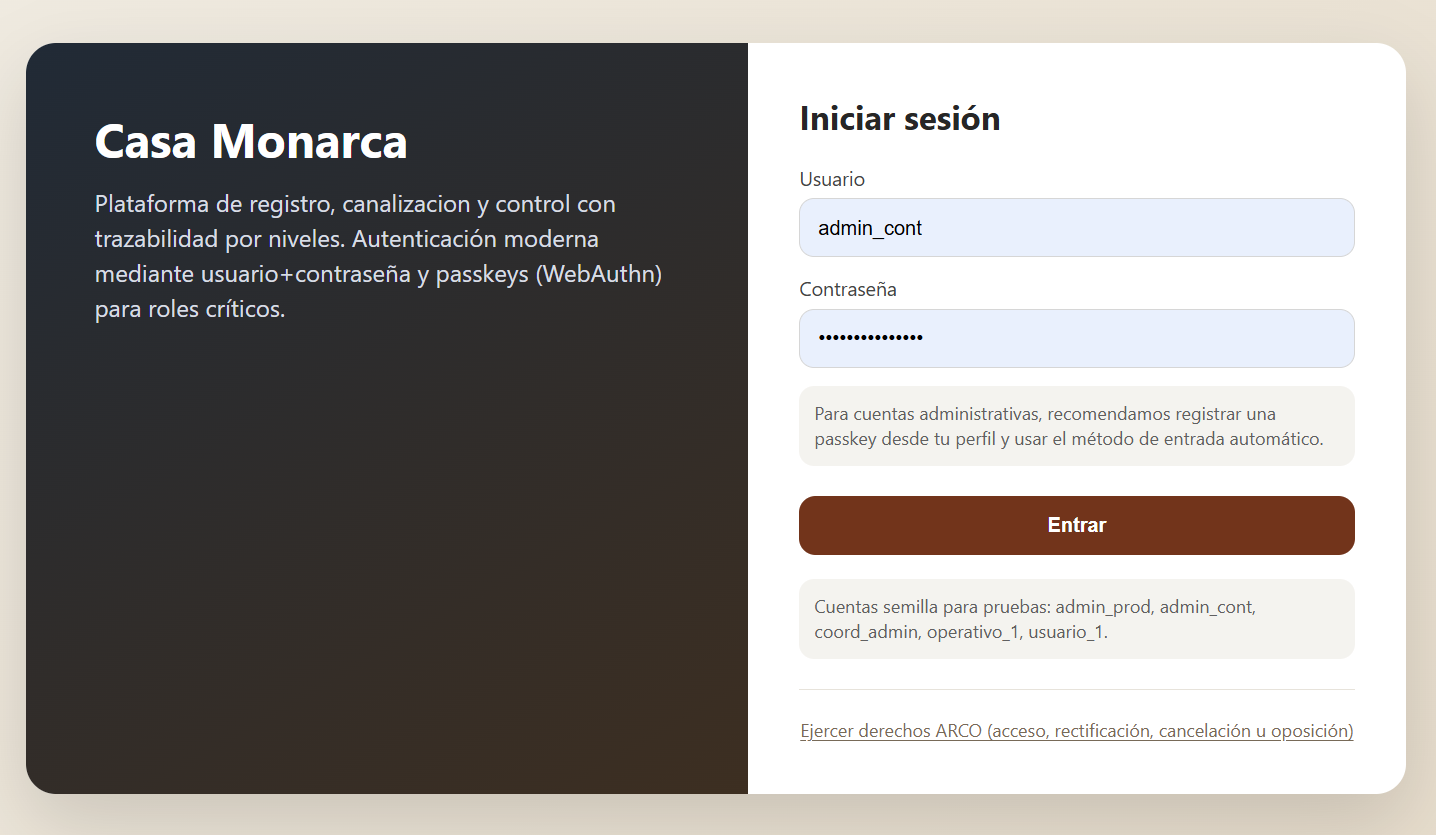
\includegraphics[width=\linewidth]{Inicio de Sesión.png}
  \end{minipage}
  \hfill
  \caption{Página de Login}
  \label{fig:login}
\end{figure}

A la hora de iniciar sesión se pedirá tanto el usuario como la contraseña
del perfil al que se busca acceder.\vspace{0.3cm}

\begin{nota}[Bloqueo por seguridad]
Tras varios intentos fallidos consecutivos, el acceso se bloquea
temporalmente como medida de protección. En ese caso deberá esperar unos
minutos antes de volver a intentarlo.
\end{nota}

\subsection{Llaves de acceso (Passkeys)}

Para mayor seguridad, los usuarios pueden iniciar sesión con una
\textbf{passkey} (huella digital, rostro o PIN del dispositivo) en lugar de
escribir la contraseña. Si su cuenta tiene una passkey registrada, aparecerá
la opción correspondiente durante el inicio de sesión.

\begin{figure}[H]
  \centering
  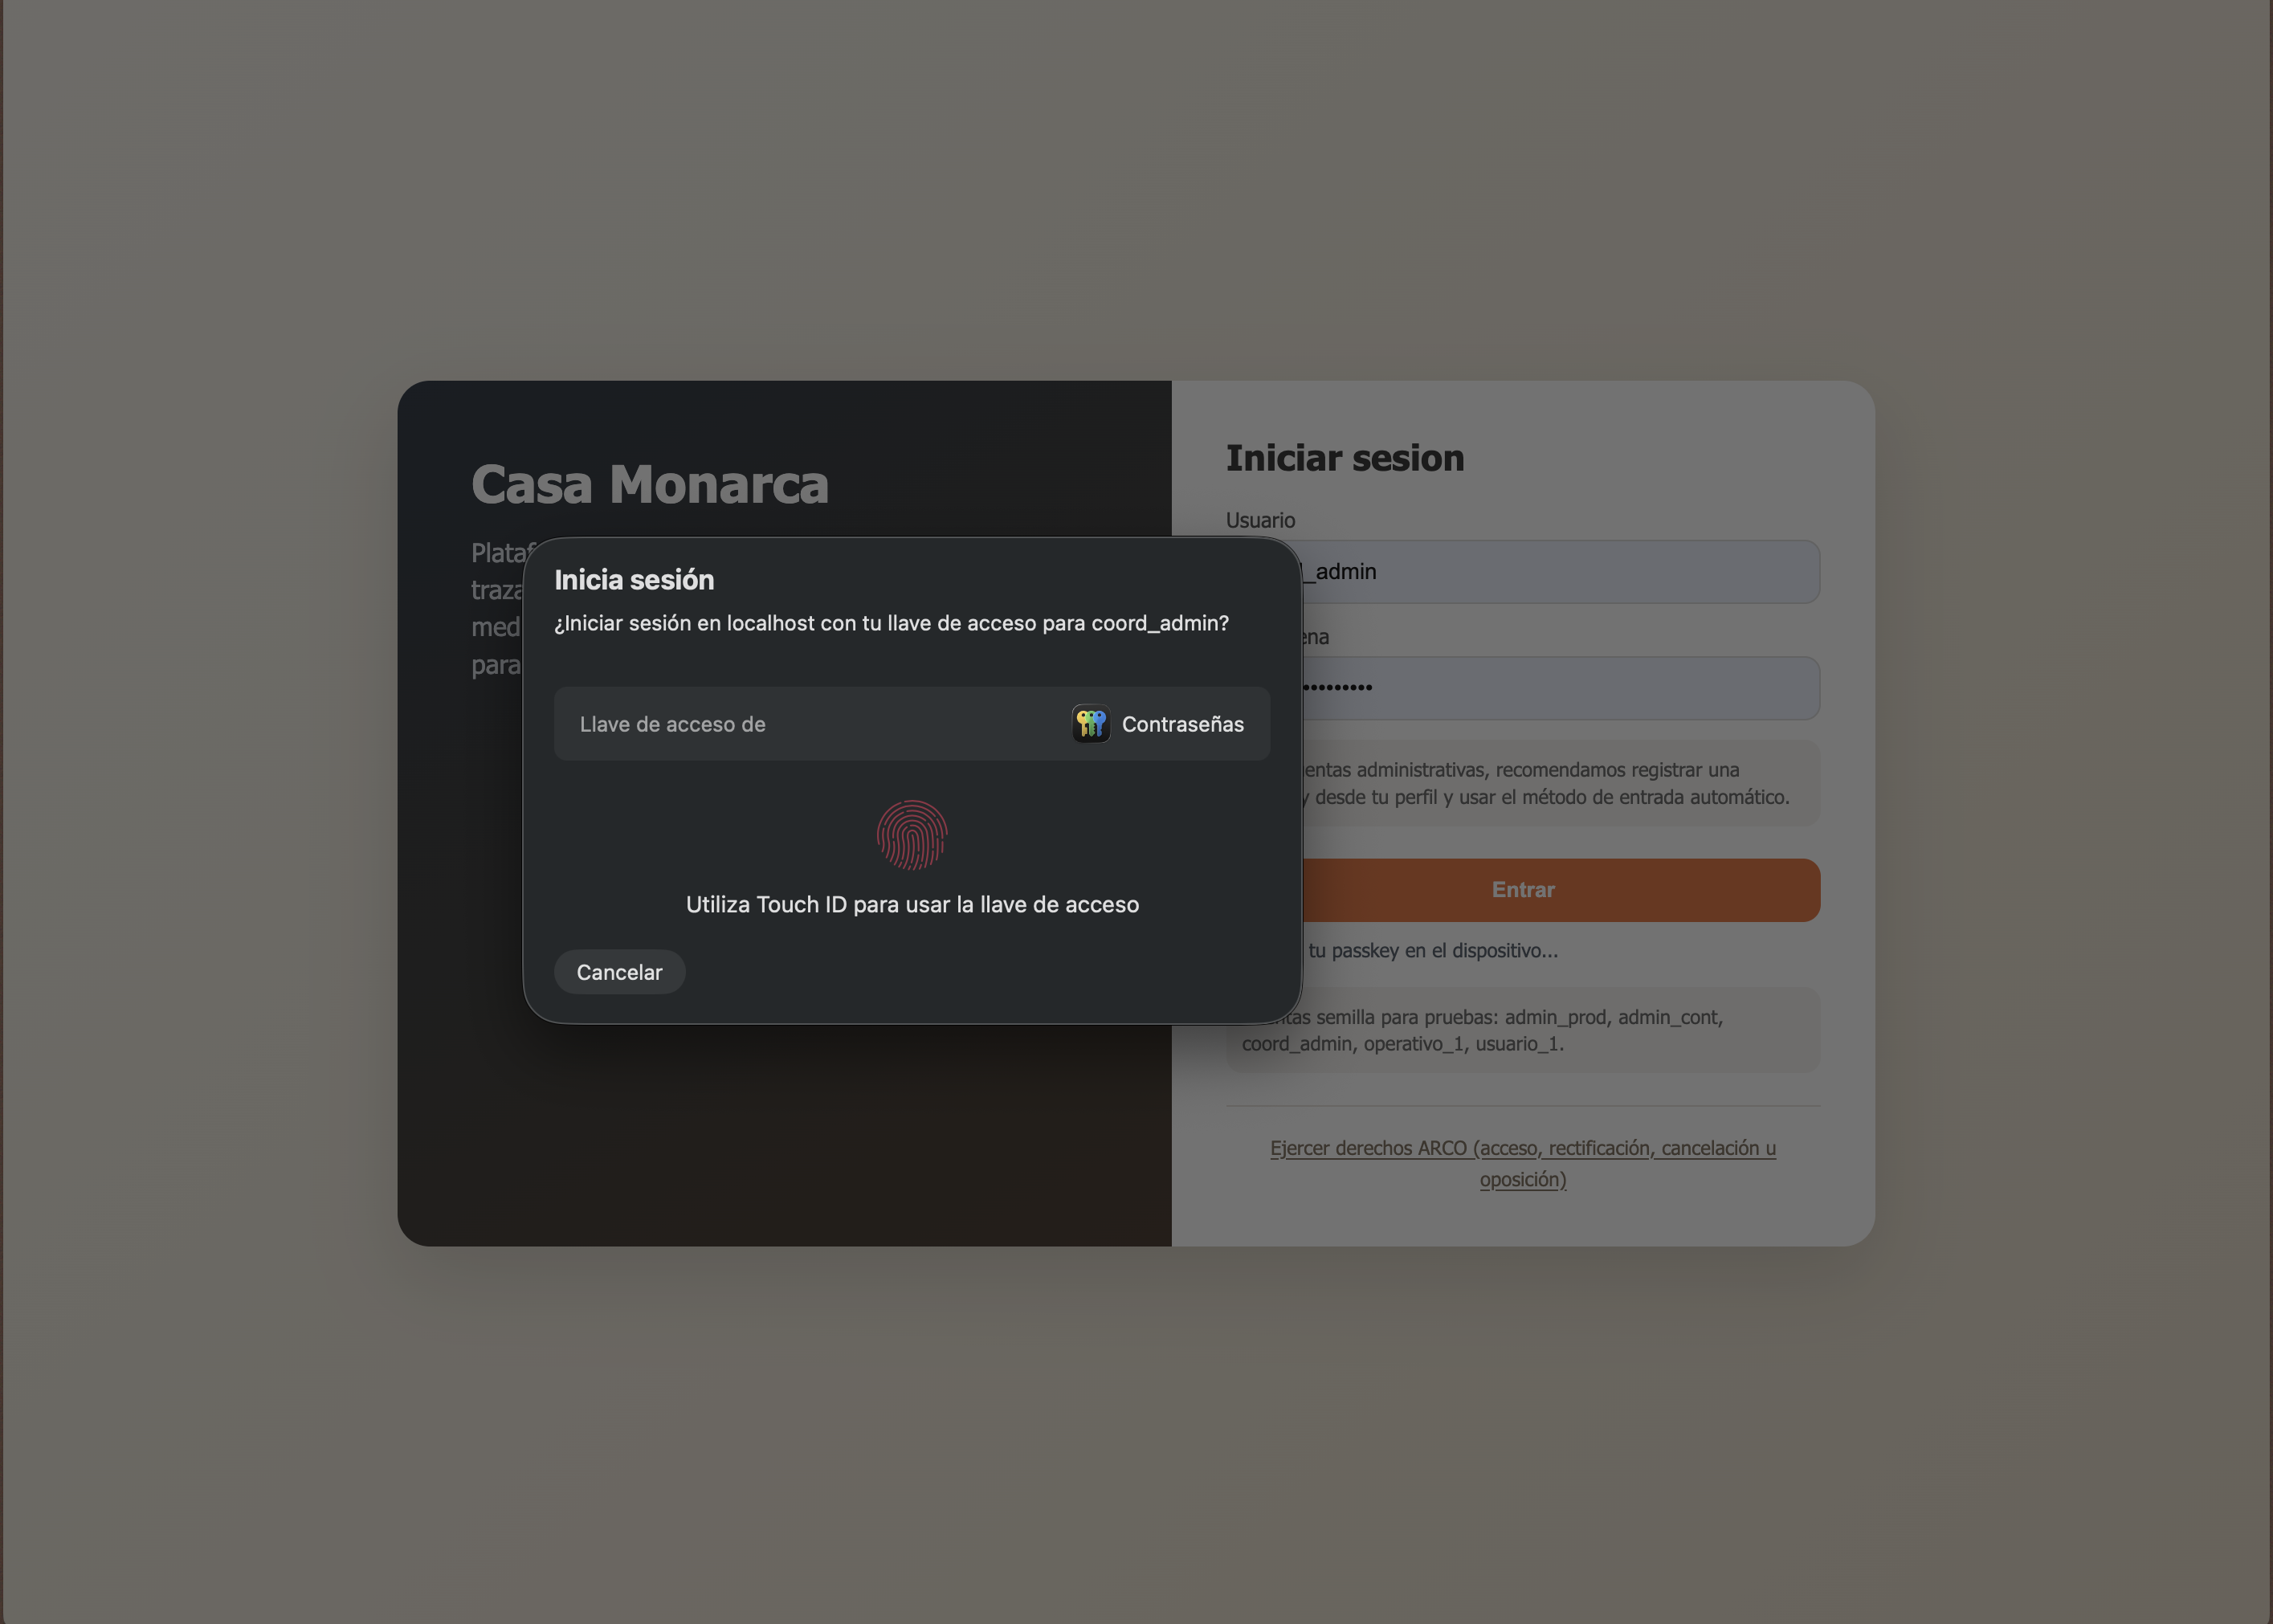
\includegraphics[width=0.48\linewidth]{Passkey.png}
  \caption{Proceso Passkey}
  \label{fig:passkey}
\end{figure}

\subsection{Cuentas con certificado digital}

Los roles críticos (Administrador y Coordinador) pueden requerir un
\textbf{certificado digital} o el registro de una passkey la primera vez que
ingresan. El sistema guiará al usuario por este proceso de configuración
cuando sea necesario.

% ════════════════════════════════════════════════════════════════════
\newpage
\section{Configuración Inicial de Seguridad}

\subsection{Cambio obligatorio de contraseña}

La primera vez que un usuario ingresa, o cuando su contraseña es considerada
insegura o caducada, el sistema solicita \textbf{actualizar la contraseña}
antes de continuar.

\begin{figure}[H]
  \centering
  \begin{minipage}{0.48\textwidth}
    \centering
    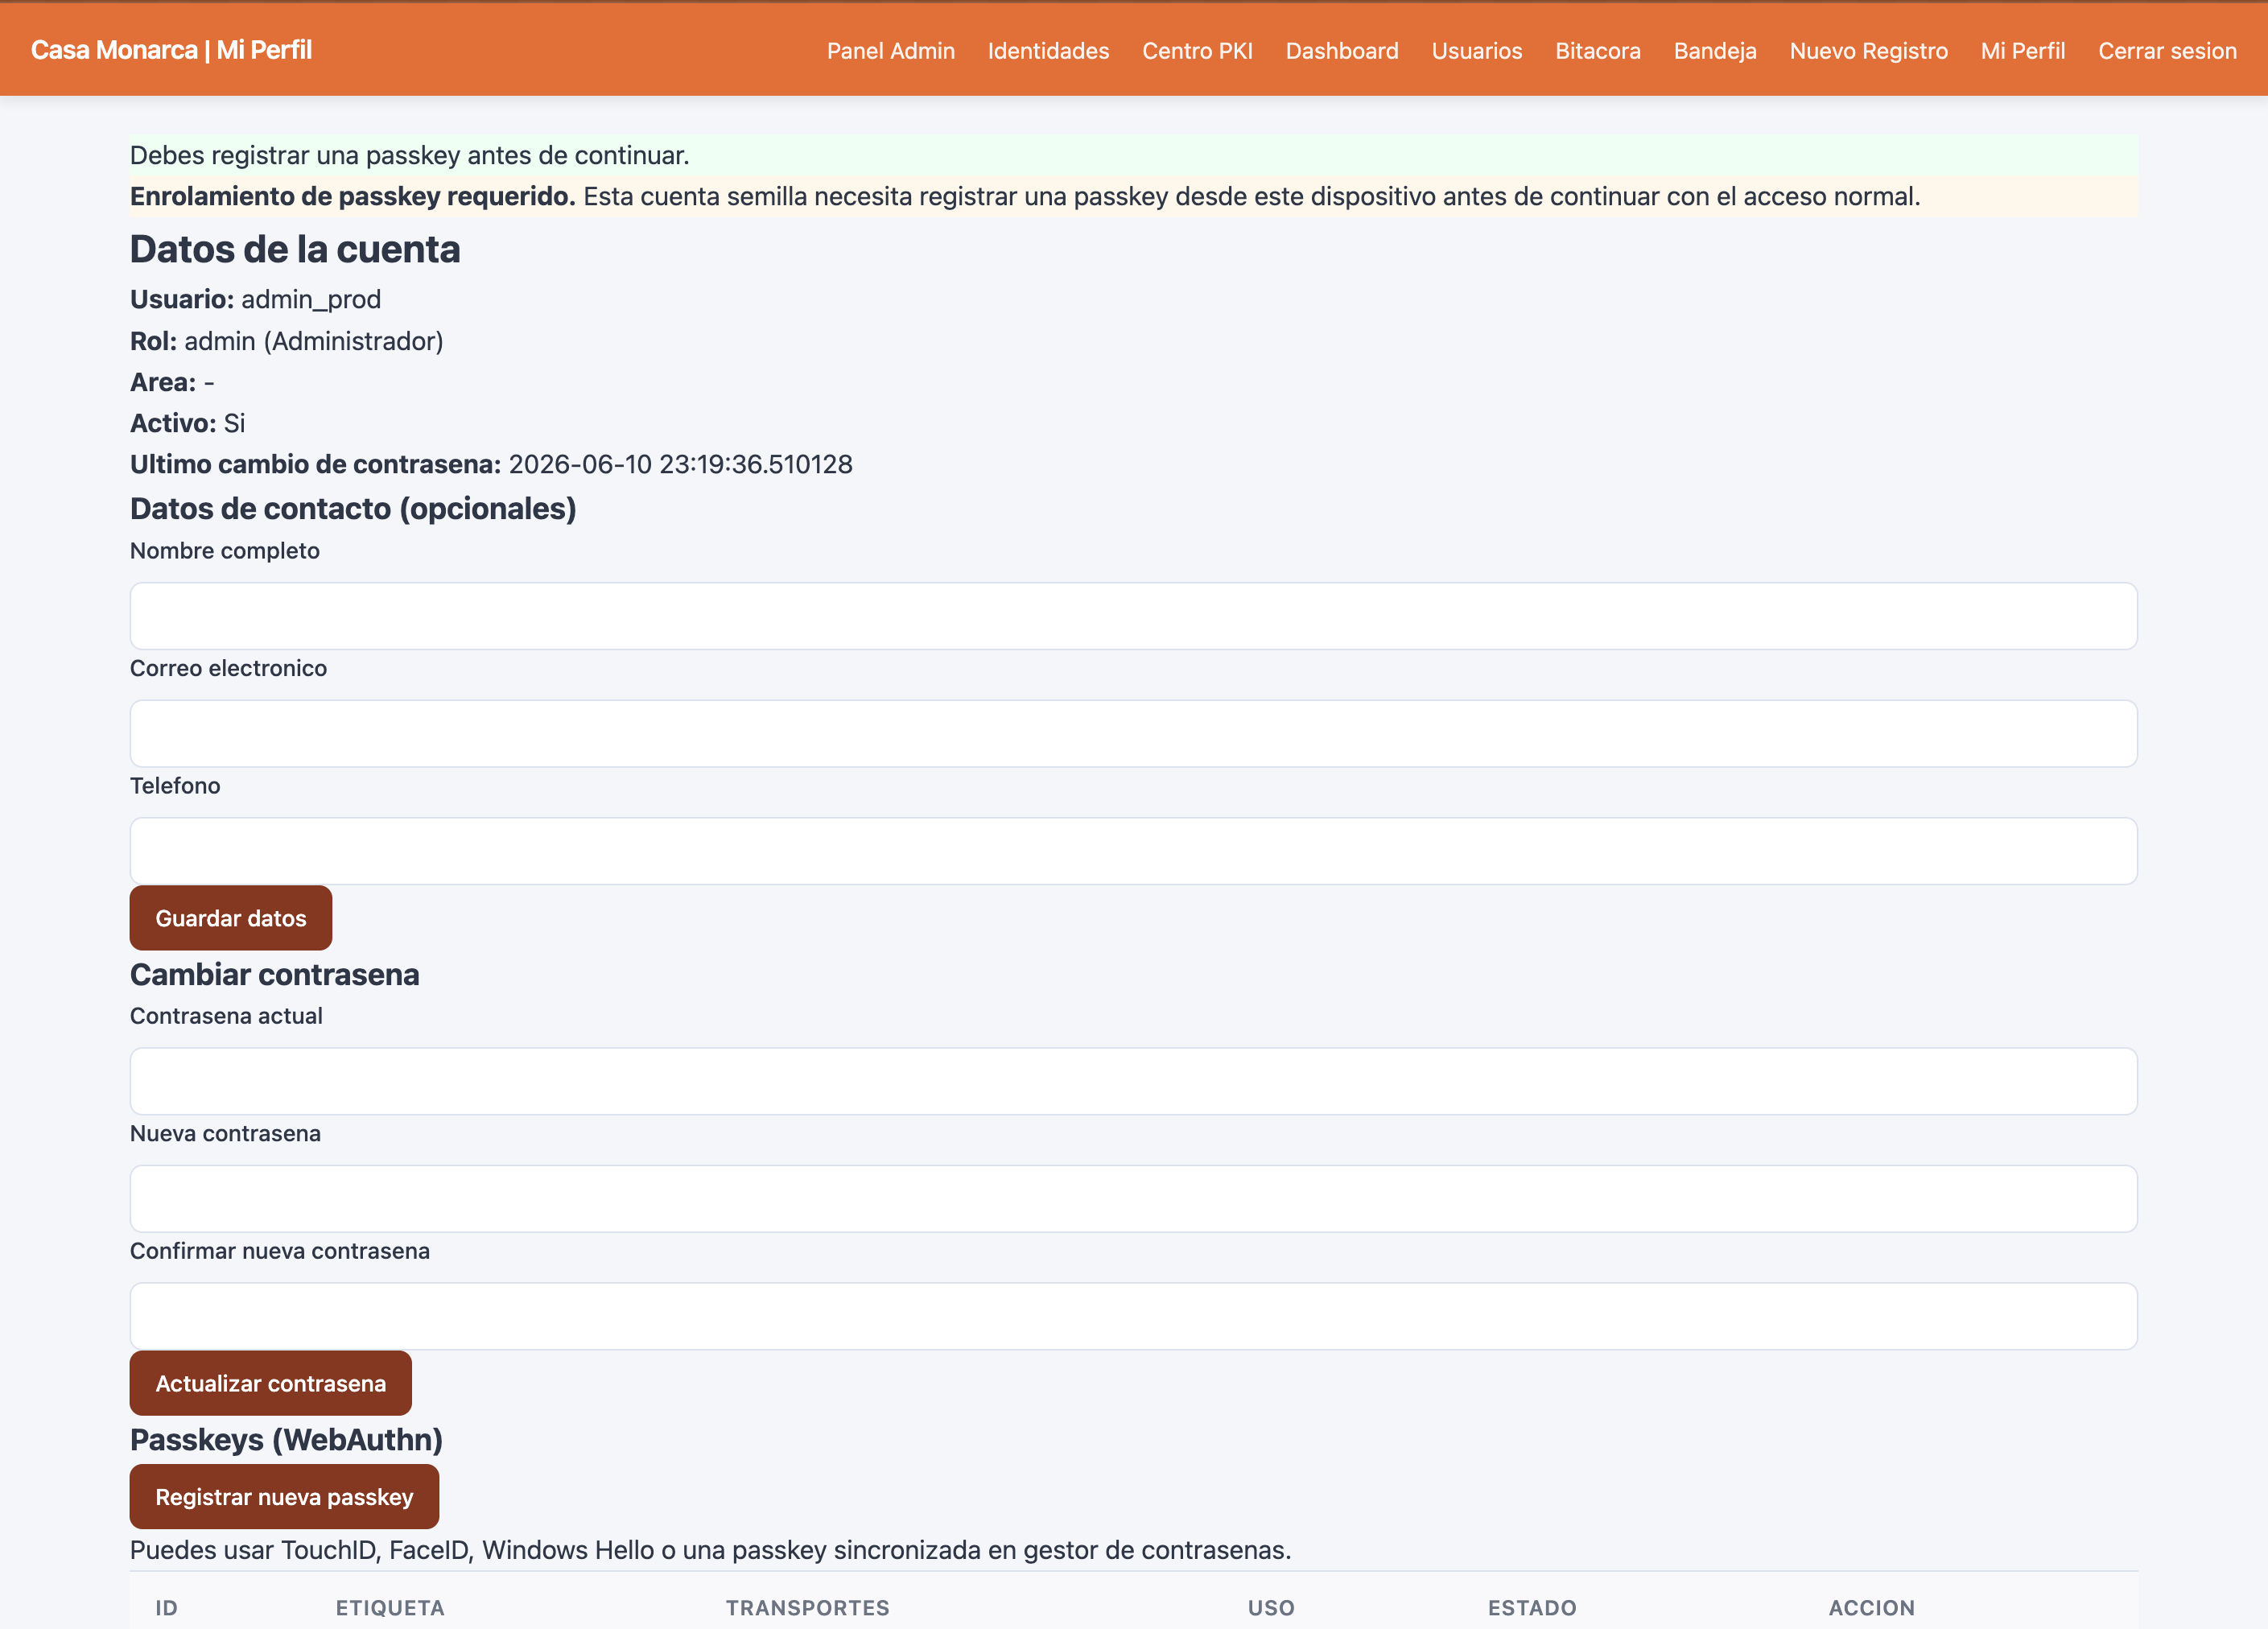
\includegraphics[width=0.8\textwidth]{Cambiocontra.png}
  \end{minipage}
  \caption{Cambio de Contraseña}
  \label{fig:cambiocontra}
\end{figure}

\begin{enumerate}[leftmargin=2em]
  \item Escriba la nueva contraseña.
  \item Confírmela en el segundo campo.
  \item Presione \textbf{Actualizar contraseña}.
\end{enumerate}

\begin{nota}[Requisitos de la contraseña]
La nueva contraseña debe tener una longitud mínima, combinar mayúsculas,
minúsculas, números y símbolos, y no aparecer en listas conocidas de
contraseñas filtradas.
\end{nota}

\subsection{Configuración del certificado digital (Admin y Coordinador)}
\label{sec:cert-setup}

Los usuarios con rol \textbf{Administrador} o \textbf{Coordinador} deben
completar la configuración de su certificado digital antes de poder usar el
sistema. Esta pantalla aparece automáticamente al primer ingreso si no existe
un certificado activo.

Existen dos formas de completar la configuración:

\begin{description}[leftmargin=2em]
  \item[Opción A — Passphrase automática]
    Ingrese una passphrase de al menos 10 caracteres y confírmela. El sistema
    generará y firmará el certificado RSA-2048 de forma automática.
  \item[Opción B — CSR propio]
    Genere una \textit{Certificate Signing Request} (CSR) en su equipo y
    cárguela en el formulario. El sistema firmará el certificado con la CA
    interna de Casa Monarca y lo descargará automáticamente en formato
    \texttt{.crt}.
\end{description}

\begin{nota}[Configuración obligatoria]
Sin completar este paso, el Administrador o Coordinador no podrá acceder a
ninguna función del sistema. El proceso se realiza una única vez por cuenta.
\end{nota}

% ════════════════════════════════════════════════════════════════════
\section{Verificación con Passkey para Acciones Sensibles}
\label{sec:passkey-action}

Ciertas acciones críticas del sistema requieren una \textbf{verificación
adicional con passkey} antes de ejecutarse, independientemente de que el
usuario ya haya iniciado sesión. Esta medida garantiza que la persona que
autoriza la acción es efectivamente quien dice ser.

\begin{nota}[Ventana de verificación]
La verificación con passkey tiene una validez de \textbf{5 minutos}. Si
intenta realizar una acción sensible y el sistema indica que la firma ha
expirado o no está disponible, deberá verificarse de nuevo antes de
continuar.
\end{nota}

Las acciones que requieren esta verificación son:

\begin{itemize}[leftmargin=2em]
  \item Resolver o rechazar solicitudes ARCO (Coordinador y Admin)
  \item Activar una nueva llave de cifrado
  \item Disparar el re-cifrado masivo de expedientes
  \item Descargar un certificado digital
  \item Revocar un certificado digital
  \item Crear cuentas con rol Administrador o Coordinador
  \item Eliminar usuarios del sistema
\end{itemize}

El sistema mostrará un botón o diálogo de verificación antes de ejecutar
cada una de estas acciones. Siga las instrucciones del dispositivo (huella,
rostro o PIN) para completar la verificación.

% ════════════════════════════════════════════════════════════════════
\section{Dashboard (Centro de Trabajo)}

El \textbf{Dashboard} o Centro de trabajo es la pantalla principal que
aparece tras iniciar sesión. Ofrece una vista rápida del estado de los
expedientes y un menú de navegación hacia el resto de las secciones.

\begin{figure}[H]
  \centering
  \begin{minipage}{0.48\textwidth}
    \centering
    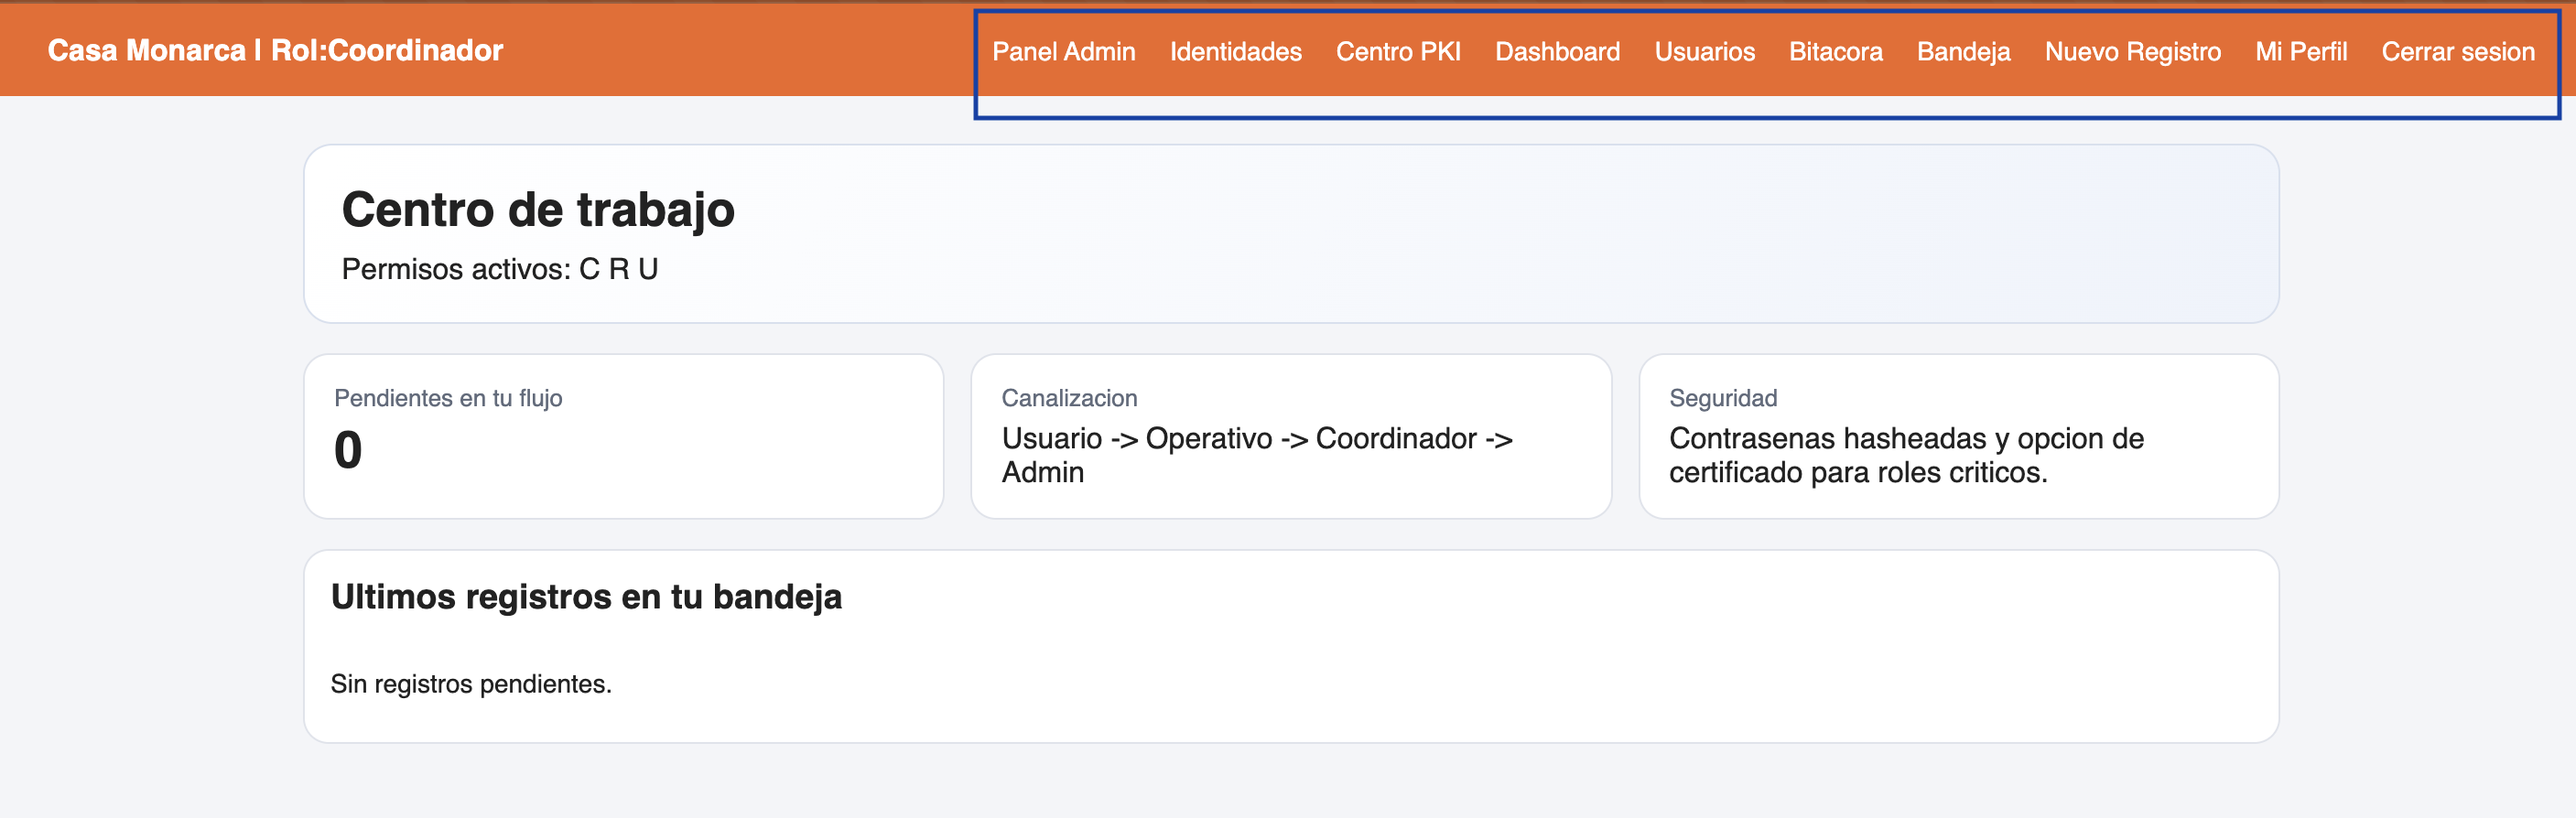
\includegraphics[width=0.8\textwidth]{Dashboard.png}
  \end{minipage}
  \caption{Visualización del Dashboard}
  \label{fig:dashboard}
\end{figure}

En la parte superior se encuentra el menú principal. Las opciones visibles
dependen del rol del usuario; en este caso el que se puede observar es del
Coordinador:

\begin{itemize}[leftmargin=2em]
  \item \textbf{Dashboard:} regresa al centro de trabajo.
  \item \textbf{Nuevo Registro:} abre el formulario para registrar un beneficiario.
  \item \textbf{Bandeja:} muestra los expedientes pendientes del usuario.
  \item \textbf{Mi Perfil:} datos personales y opciones de seguridad.
  \item \textbf{Panel Admin:} (solo administradores) gestión global de expedientes.
  \item \textbf{Usuarios:} (administradores) alta y baja de cuentas.
  \item \textbf{Identidades:} (administradores) resumen de identidades.
  \item \textbf{Centro PKI:} (administradores) gestión de certificados.
  \item \textbf{Cifrado:} (administradores y coordinadores) gestión de llaves de cifrado.
  \item \textbf{Bitácora:} historial de eventos del sistema.
  \item \textbf{Cerrar sesión:} sale de la cuenta de forma segura.
\end{itemize}

\subsection{Últimos registros en la bandeja}

La pantalla muestra una lista de los \textbf{últimos registros} asignados al
usuario, con su número de expediente y estado actual, para acceder a ellos
rápidamente.

\begin{figure}[H]
  \centering
  \begin{minipage}{0.48\textwidth}
    \centering
    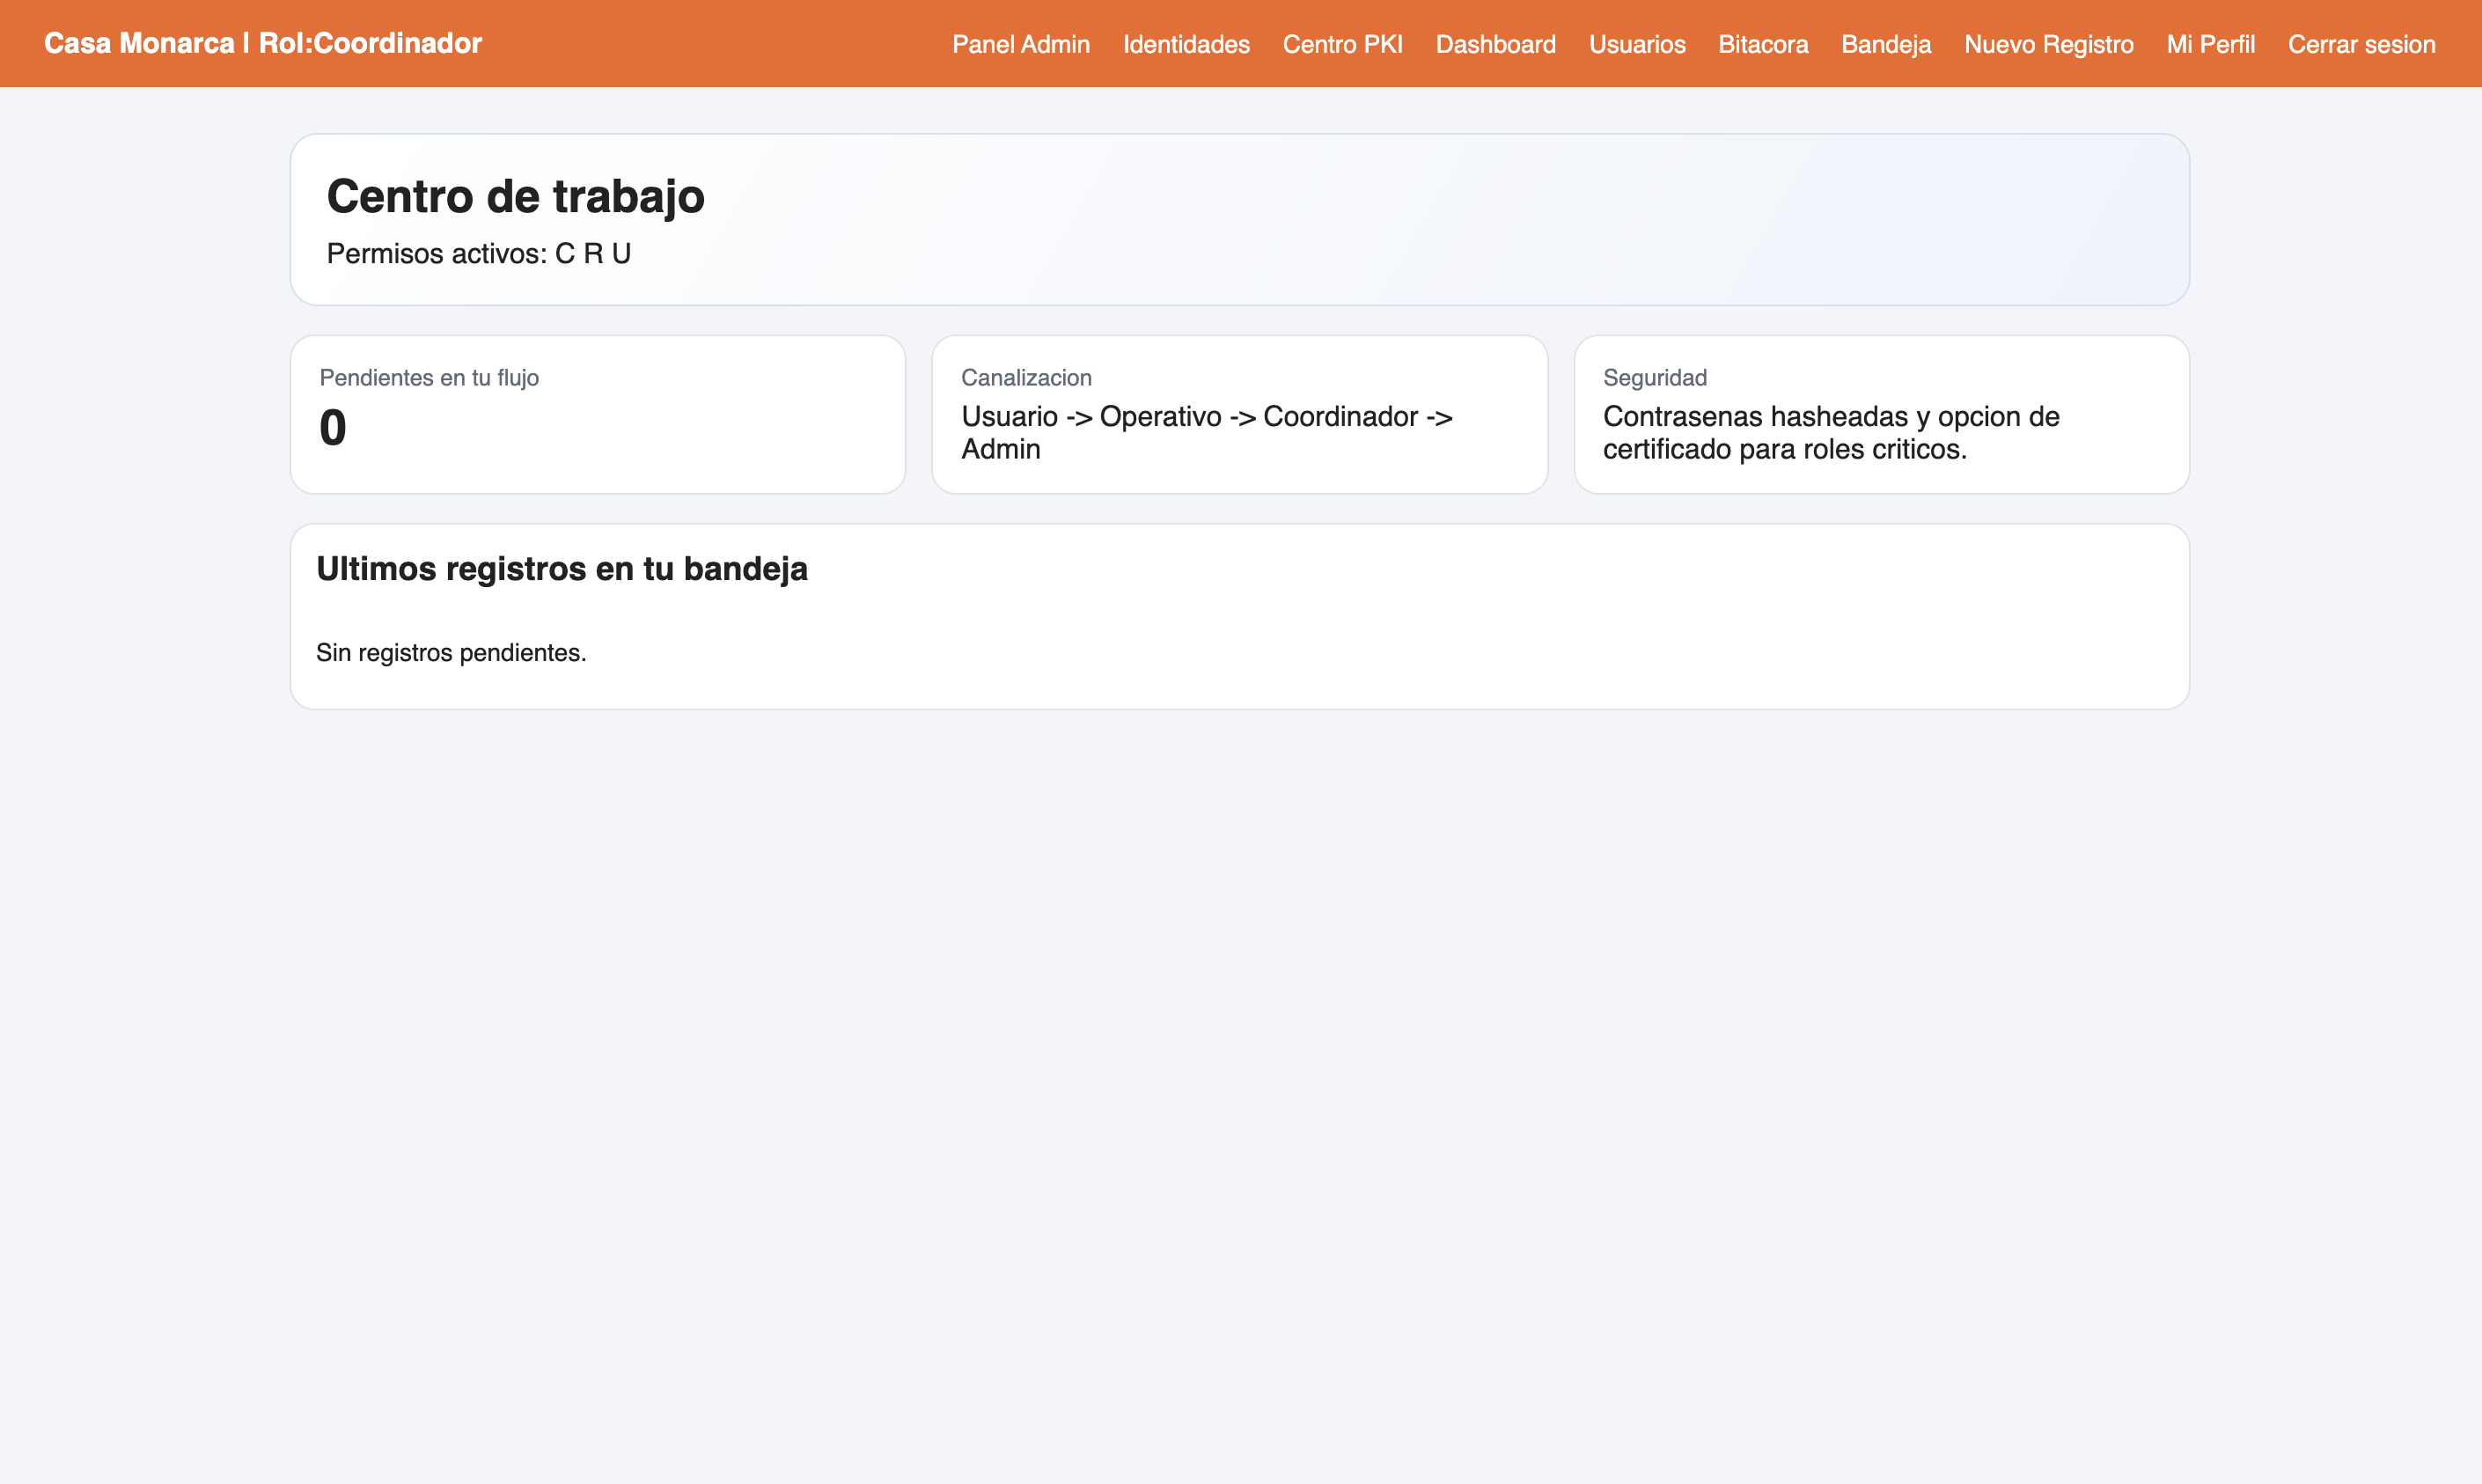
\includegraphics[width=0.8\textwidth]{Bandeja.png}
  \end{minipage}
  \caption{Visualización de la Bandeja}
  \label{fig:bandeja-dashboard}
\end{figure}

% ════════════════════════════════════════════════════════════════════
\section{Registros de Beneficiarios}


La opción \textbf{Nuevo Registro} abre el formulario para dar de alta a una
persona beneficiaria. Es el punto de entrada de información al sistema.

\subsubsection{Campos del formulario}

\begin{figure}[H]
  \centering
  \begin{minipage}{0.48\textwidth}
    \centering
    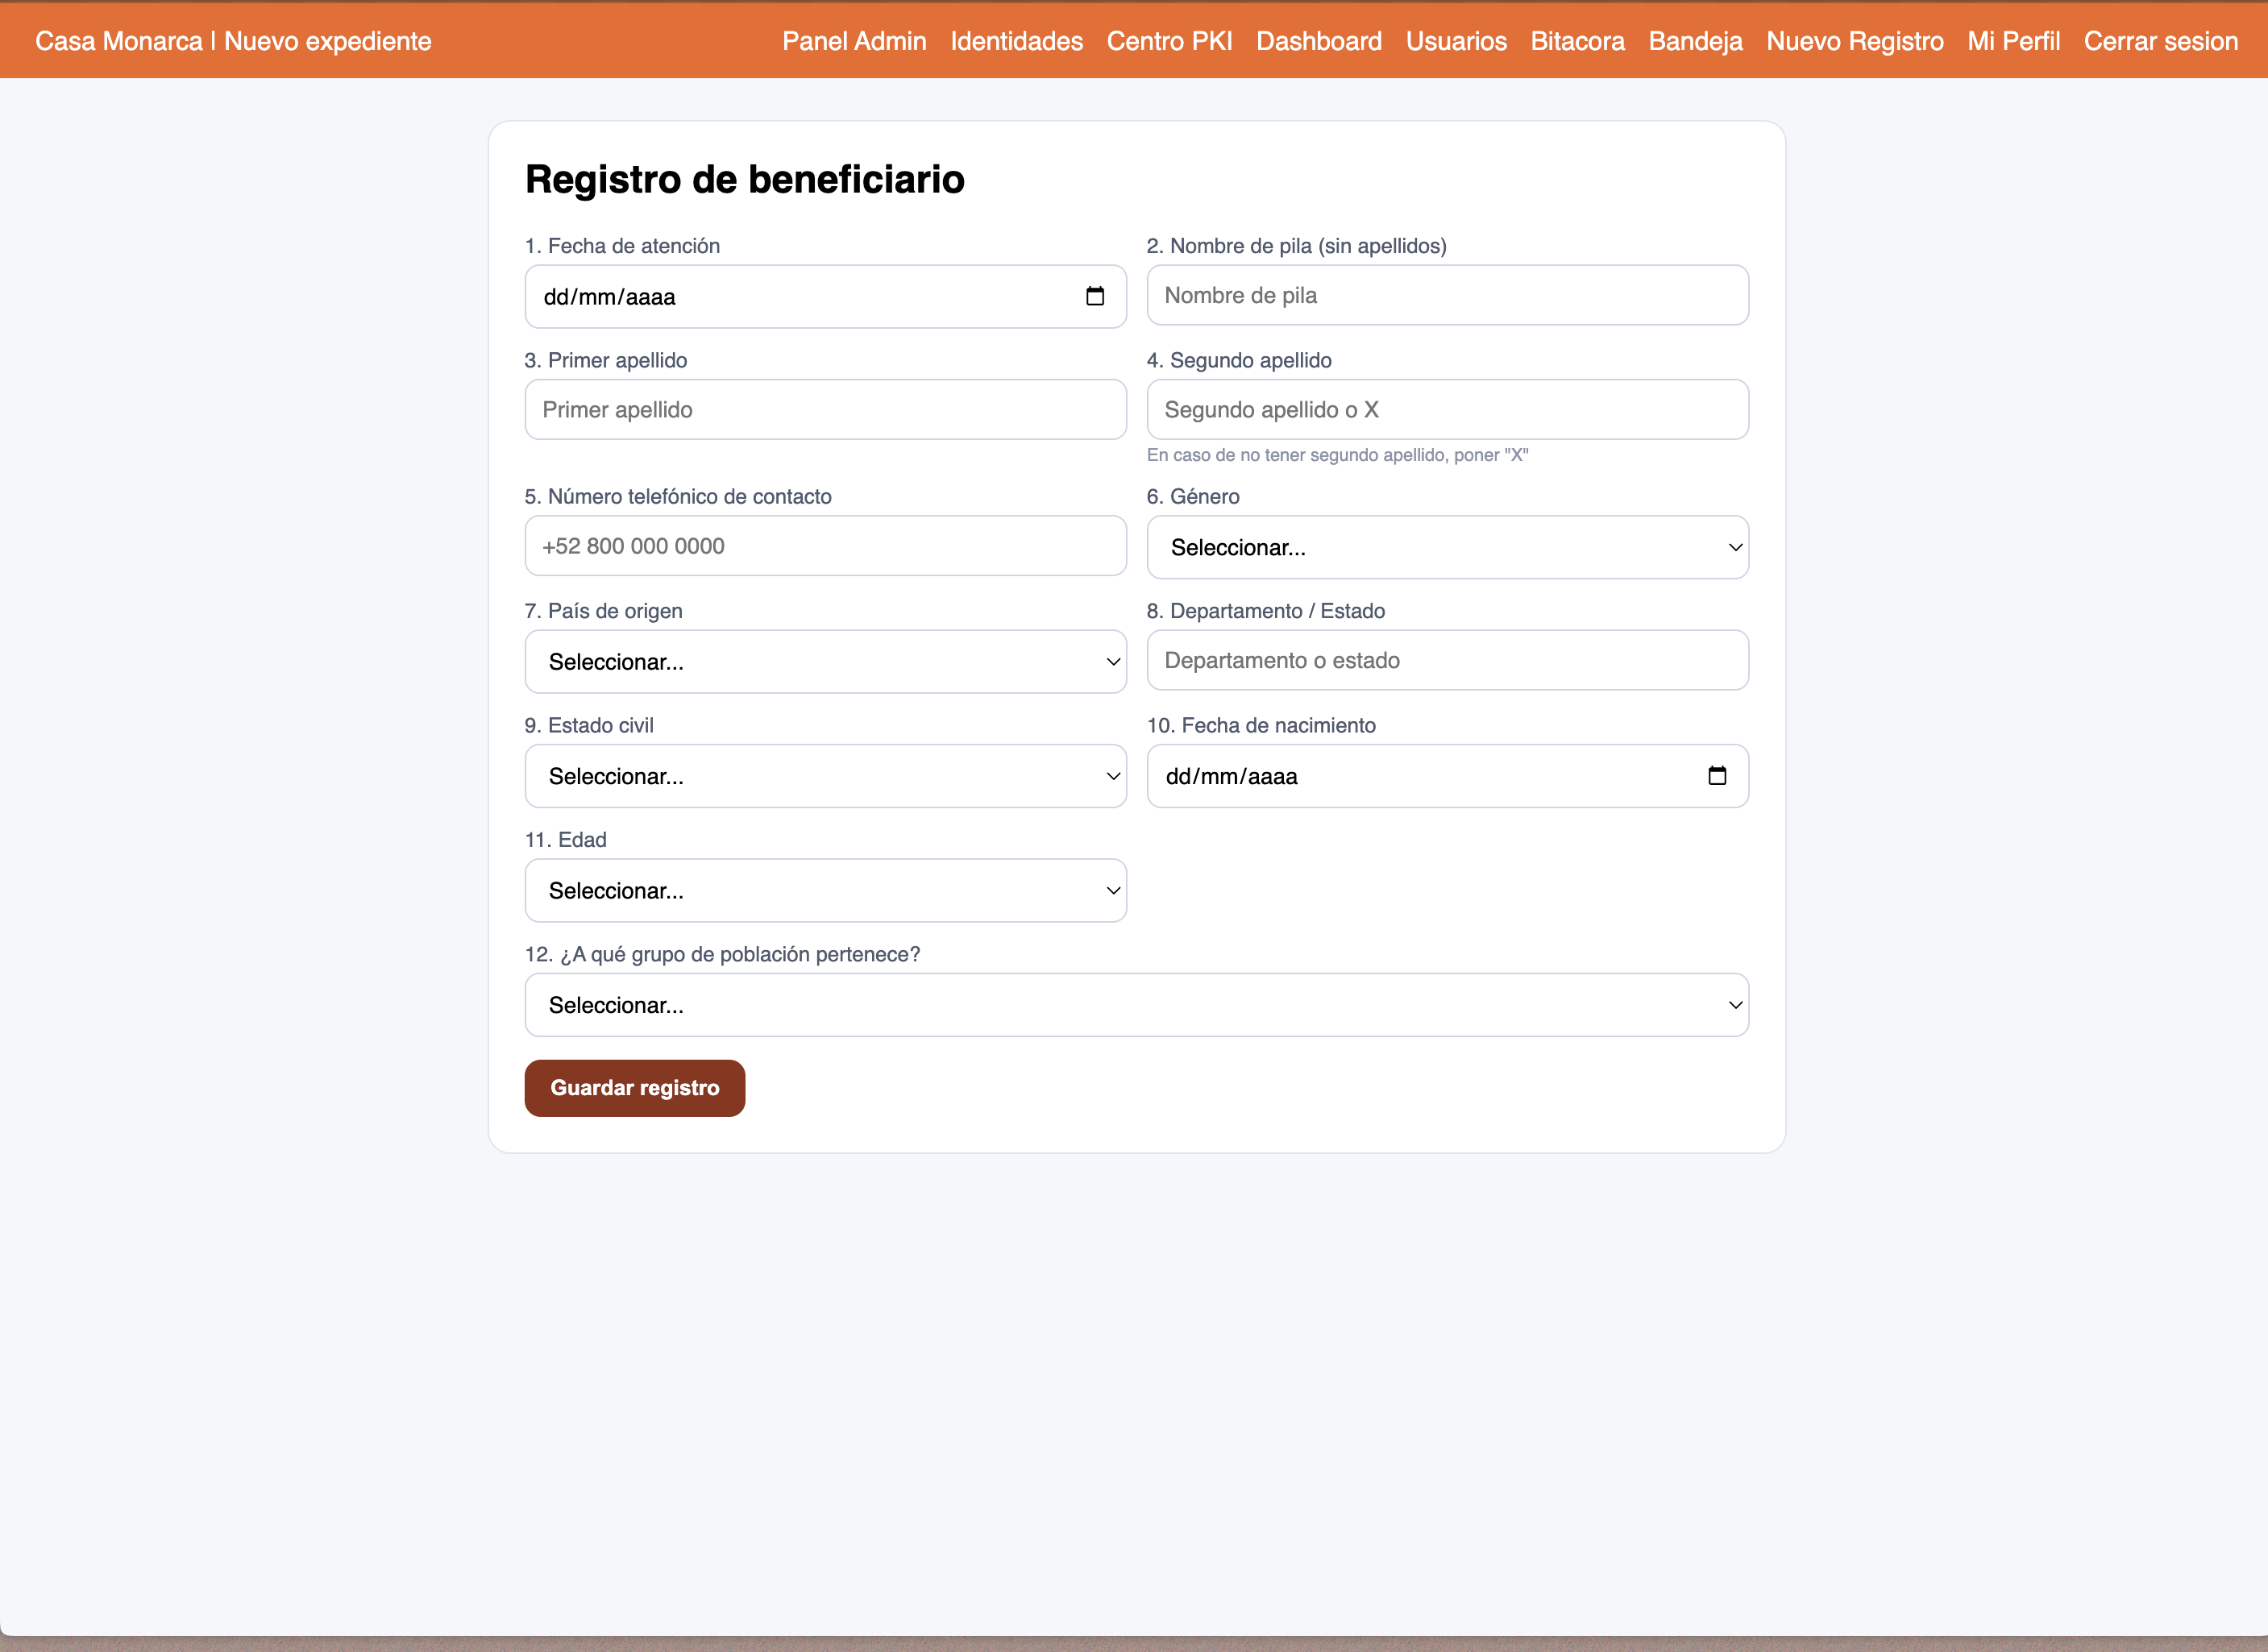
\includegraphics[width=0.8\textwidth]{CamposRegistro.png}
  \end{minipage}
  \caption{Visualización de los campos del formulario}
  \label{fig:campos-registro}
\end{figure}

El formulario recoge los datos básicos de la persona:

\begin{itemize}[leftmargin=2em]
  \item \textbf{Nombre de pila}, \textbf{primer apellido} y \textbf{segundo apellido}.
  \item \textbf{Fecha de nacimiento} y \textbf{edad}.
  \item \textbf{Género} y \textbf{estado civil}.
  \item \textbf{País de origen} y \textbf{departamento o estado}.
  \item \textbf{Grupo de población} al que pertenece.
  \item \textbf{Teléfono} de contacto.
  \item \textbf{Fecha de atención}.
\end{itemize}

\subsubsection{Guardar el registro}

Una vez completados los campos, presione \textbf{Guardar registro}. El
expediente se almacena de forma cifrada y queda disponible en la bandeja de
trabajo para continuar su atención.

\begin{nota}[Protección de datos]
La información sensible del beneficiario se guarda cifrada con AES-256. Solo
los usuarios autorizados pueden consultarla a través de la plataforma.
\end{nota}

% ════════════════════════════════════════════════════════════════════
\section{Bandeja de Trabajo y Flujo de Expedientes}

La \textbf{Bandeja de trabajo} muestra los expedientes que están a cargo del
usuario y permite avanzarlos a través de los distintos niveles de atención.

\subsection{Tarjeta de expediente}

Cada expediente se presenta como una tarjeta que indica su número, el nombre
del beneficiario y su estado actual. Desde la tarjeta se realizan las
acciones de canalización.

\subsection{Flujo de canalización}

Los expedientes recorren un flujo por niveles. Según su rol y el estado del
expediente, el usuario verá disponibles algunas de estas acciones:

\begin{description}[leftmargin=2em]
  \item[Canalizar a Operativo] Envía el expediente al siguiente nivel de atención.
  \item[Canalizar a Coordinador] Eleva el expediente al coordinador del área.
  \item[Validar y enviar a Admin] El coordinador valida y remite al administrador.
  \item[Cerrar expediente] El administrador da por concluido el caso.
  \item[Solicitar eliminación] Genera una solicitud para que un administrador
    elimine el expediente.
\end{description}

\begin{nota}[Recorrido típico]
Usuario crea el expediente $\rightarrow$ se canaliza a Operativo $\rightarrow$
se canaliza a Coordinador $\rightarrow$ el Coordinador valida $\rightarrow$
el Administrador lo cierra.
\end{nota}

\begin{figure}[H]
  \centering
  \begin{minipage}{0.48\textwidth}
    \centering
    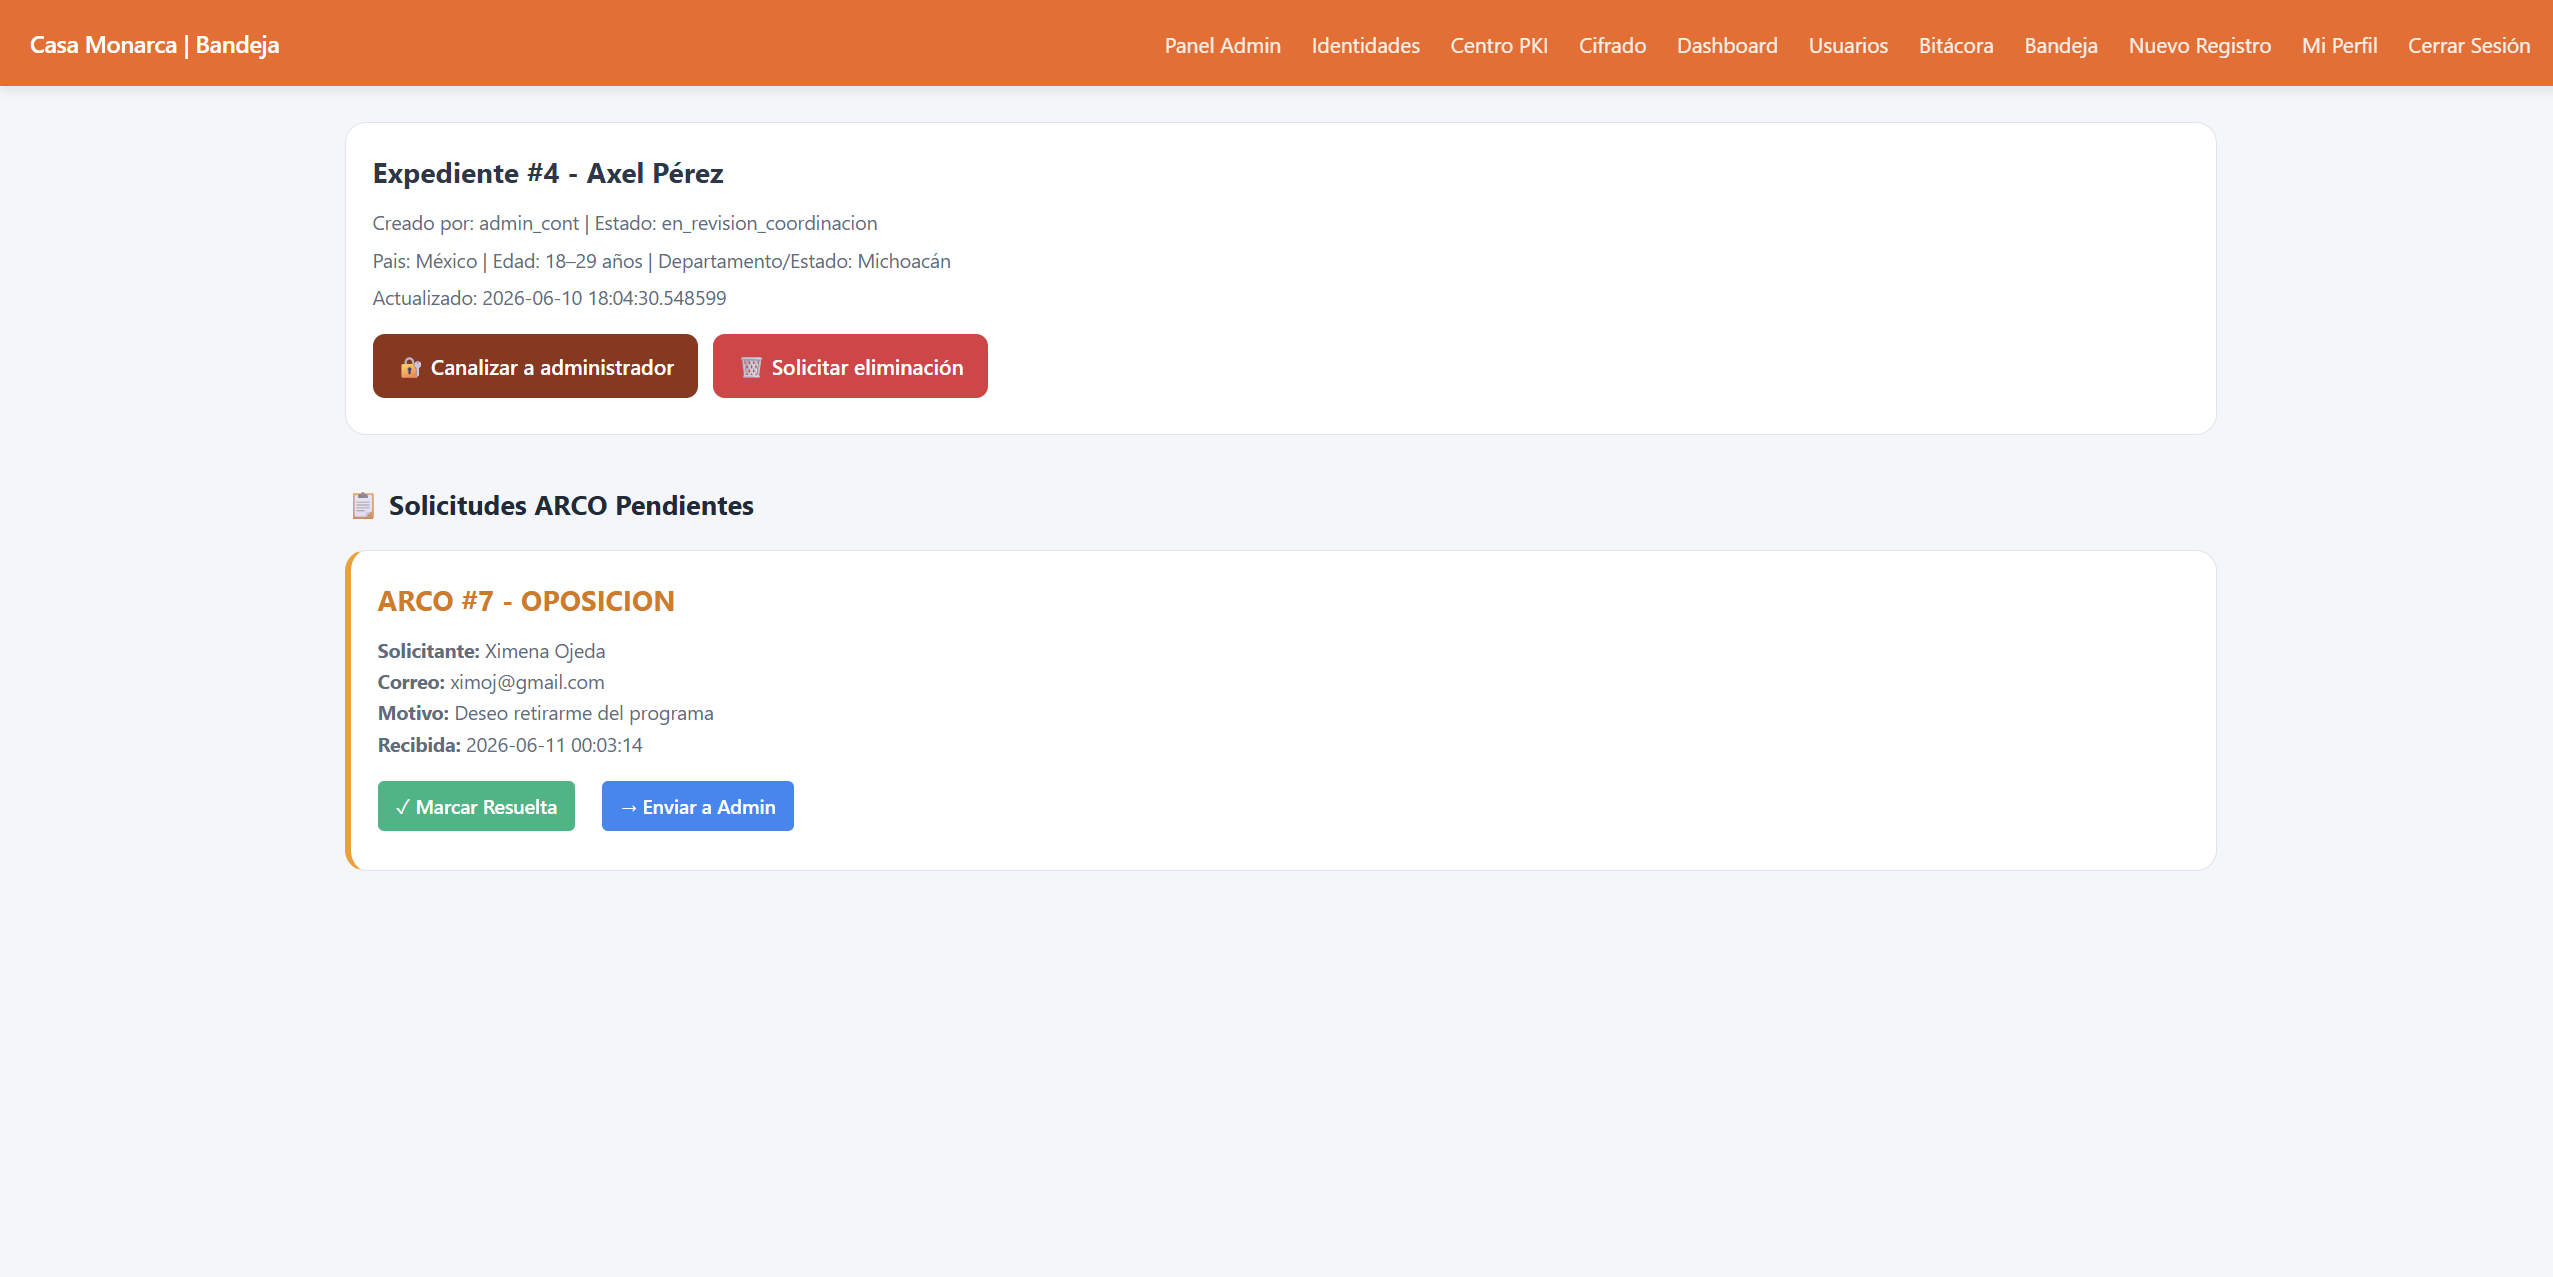
\includegraphics[width=0.8\textwidth]{Canalización Bandeja.png}
  \end{minipage}
  \caption{Ejemplo Canalización Coordinador -- Admin}
  \label{fig:canalizacion}
\end{figure}

% ════════════════════════════════════════════════════════════════════
\section{Solicitudes ARCO}
\label{sec:arco}

El sistema gestiona los derechos de protección de datos personales conforme
a la Ley Federal de Protección de Datos Personales en Posesión de los
Particulares (LFPDPPP). Los cuatro tipos de solicitudes disponibles son:

\begin{description}[leftmargin=2em]
  \item[Acceso] Conocer qué datos personales están registrados.
  \item[Rectificación] Corregir datos incorrectos o incompletos.
  \item[Cancelación] Solicitar la eliminación de datos que ya no sean necesarios.
  \item[Oposición] Oponerse al tratamiento de datos en determinados casos.
\end{description}

\begin{figure}[H]
  \centering
  \begin{minipage}{0.48\textwidth}
    \centering
    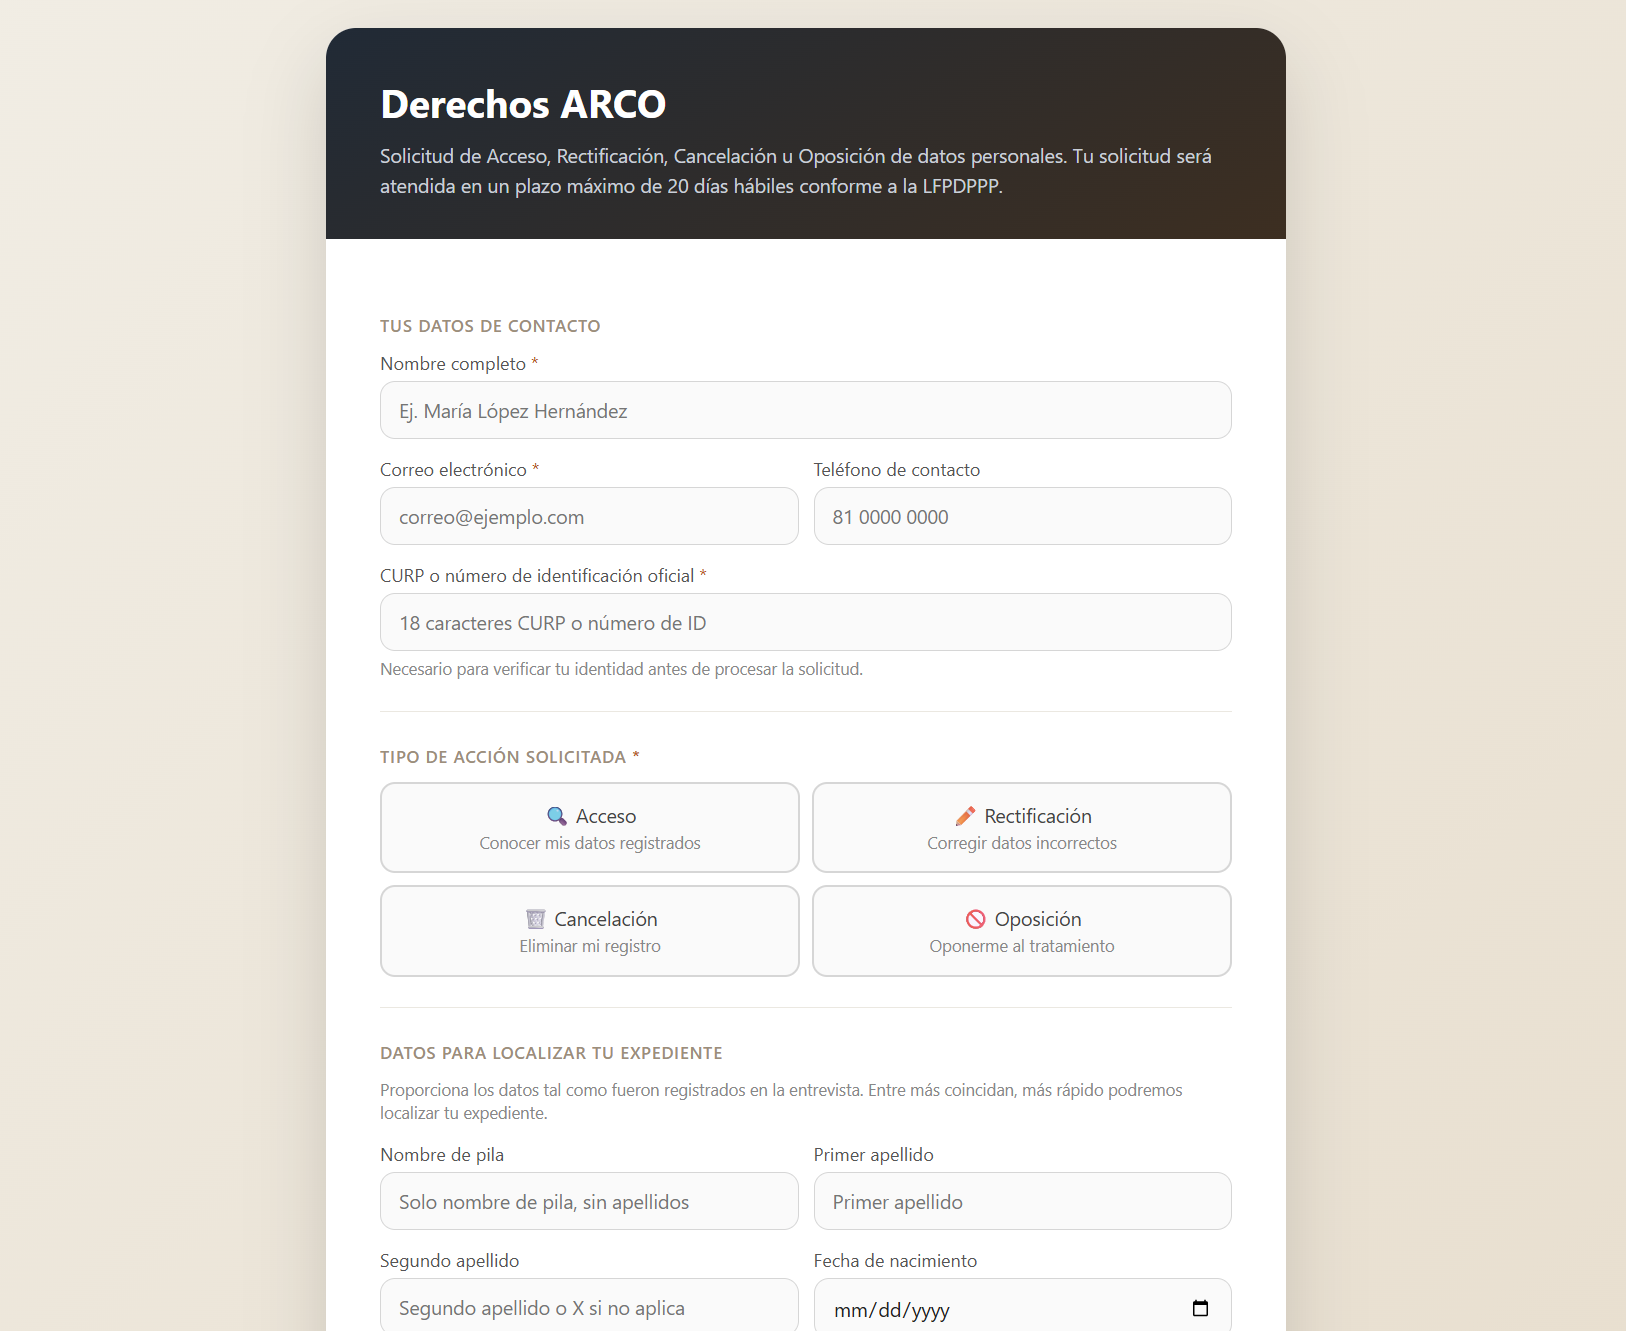
\includegraphics[width=0.8\textwidth]{Solicitud Derechos ARCO.png}
  \end{minipage}
  \caption{Solicitudes Arco}
  \label{fig:campos-registro}
\end{figure}

\subsection{Presentar una solicitud (público externo)}

Cualquier persona puede presentar una solicitud ARCO en la sección pública
del sistema (\texttt{/arco}) sin necesidad de una cuenta. Los campos
requeridos son:

\begin{itemize}[leftmargin=2em]
  \item Nombre completo del solicitante.
  \item Correo electrónico de contacto.
  \item CURP o número de identificación.
  \item Tipo de acción solicitada (Acceso, Rectificación, Cancelación u Oposición).
  \item Motivo detallado de la solicitud.
\end{itemize}

\begin{nota}[Tiempo de respuesta]
Una vez registrada, la solicitud recibirá respuesta en un plazo máximo de
\textbf{20 días hábiles}, conforme a la normativa aplicable.
\end{nota}

\subsection{Flujo interno de atención ARCO}

Las solicitudes ARCO siguen un flujo de aprobación multinivel similar al de
los expedientes. Cada rol ve en su bandeja las solicitudes que le corresponde
atender:

\begin{description}[leftmargin=2em]
  \item[Usuario y Operativo] Pueden \textbf{aprobar} la solicitud desde la
    bandeja para avanzarla al siguiente nivel.
  \item[Coordinador] Tiene tres opciones disponibles, todas requieren
    \textbf{verificación con passkey} (véase sección~\ref{sec:passkey-action}):
    \begin{itemize}
      \item \textbf{Aprobar}: avanza la solicitud al nivel admin.
      \item \textbf{Resolver directamente}: cierra la solicitud sin escalar.
      \item \textbf{Enviar como prioritaria}: eleva la solicitud al admin con
        bandera de urgencia.
    \end{itemize}
  \item[Administrador] Tiene la resolución final y dispone de los botones
    \textbf{Marcar atendida} y \textbf{Rechazar}. Estas acciones también
    requieren verificación con passkey.
\end{description}

\subsection{Solicitudes ARCO en el mainistración}

El Panel Admin agrupa las solicitudes ARCO en dos bloques:

\begin{itemize}[leftmargin=2em]
  \item \textbf{ARCO Prioritarias:} provenientes de coordinadores; requieren
    atención preferente.
  \item \textbf{ARCO (flujo directo):} solicitudes que llegaron sin ser
    escaladas como prioritarias.
\end{itemize}

\begin{figure}[H]
  \centering
  \begin{minipage}{0.48\textwidth}
    \centering
    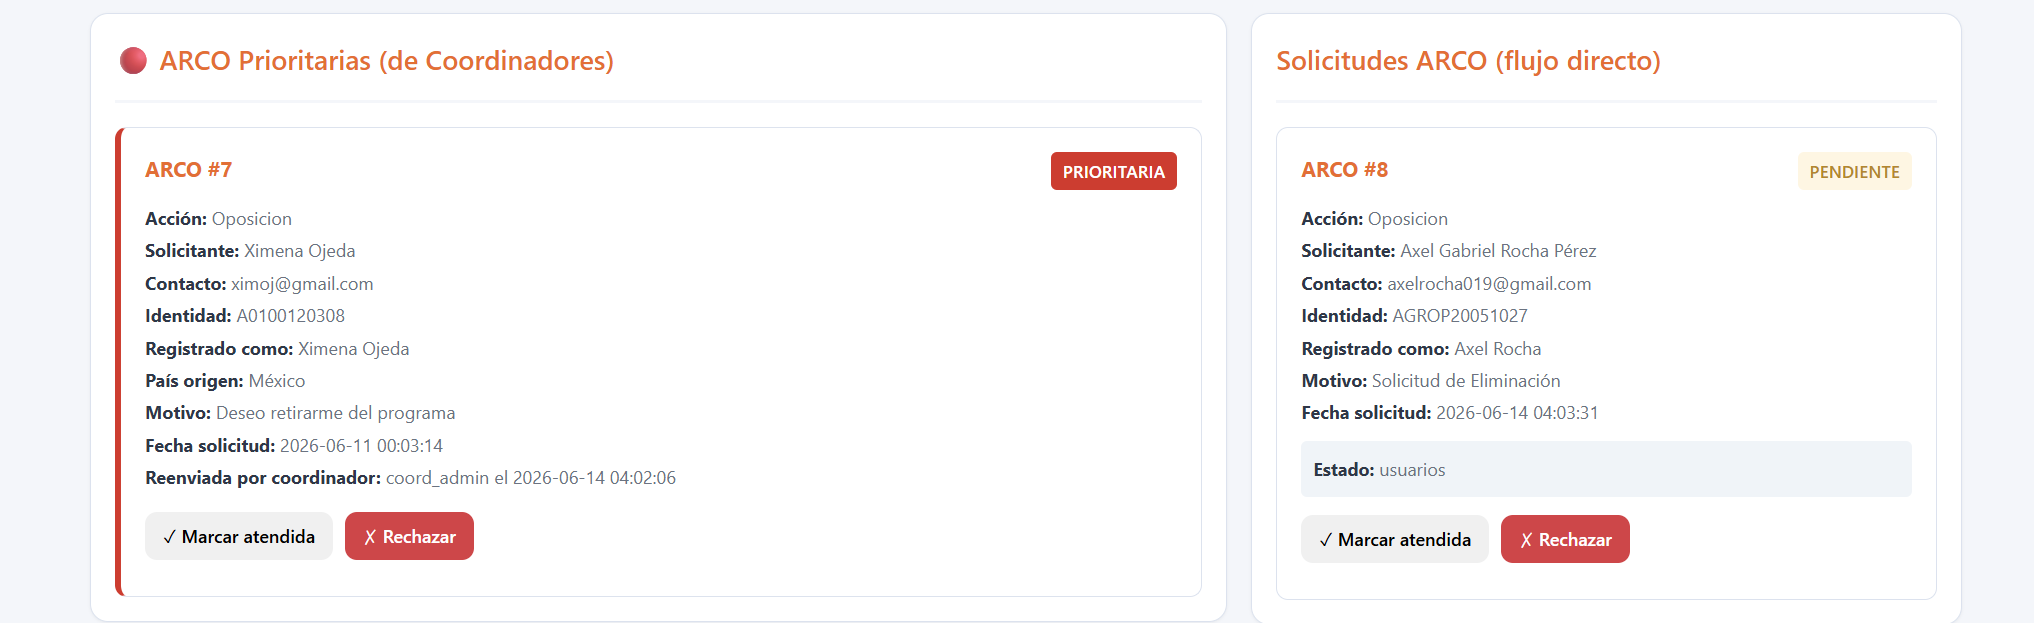
\includegraphics[width=0.8\textwidth]{Solicitudes Arcos2Flujos.png}
  \end{minipage}
  \caption{2 Flujos de Solicitudes ARCO}
  \label{fig:arco-flujos}
\end{figure}

% ════════════════════════════════════════════════════════════════════
\section{Panel Admin}

\begin{figure}[H]
  \centering
  \begin{minipage}{0.48\textwidth}
    \centering
    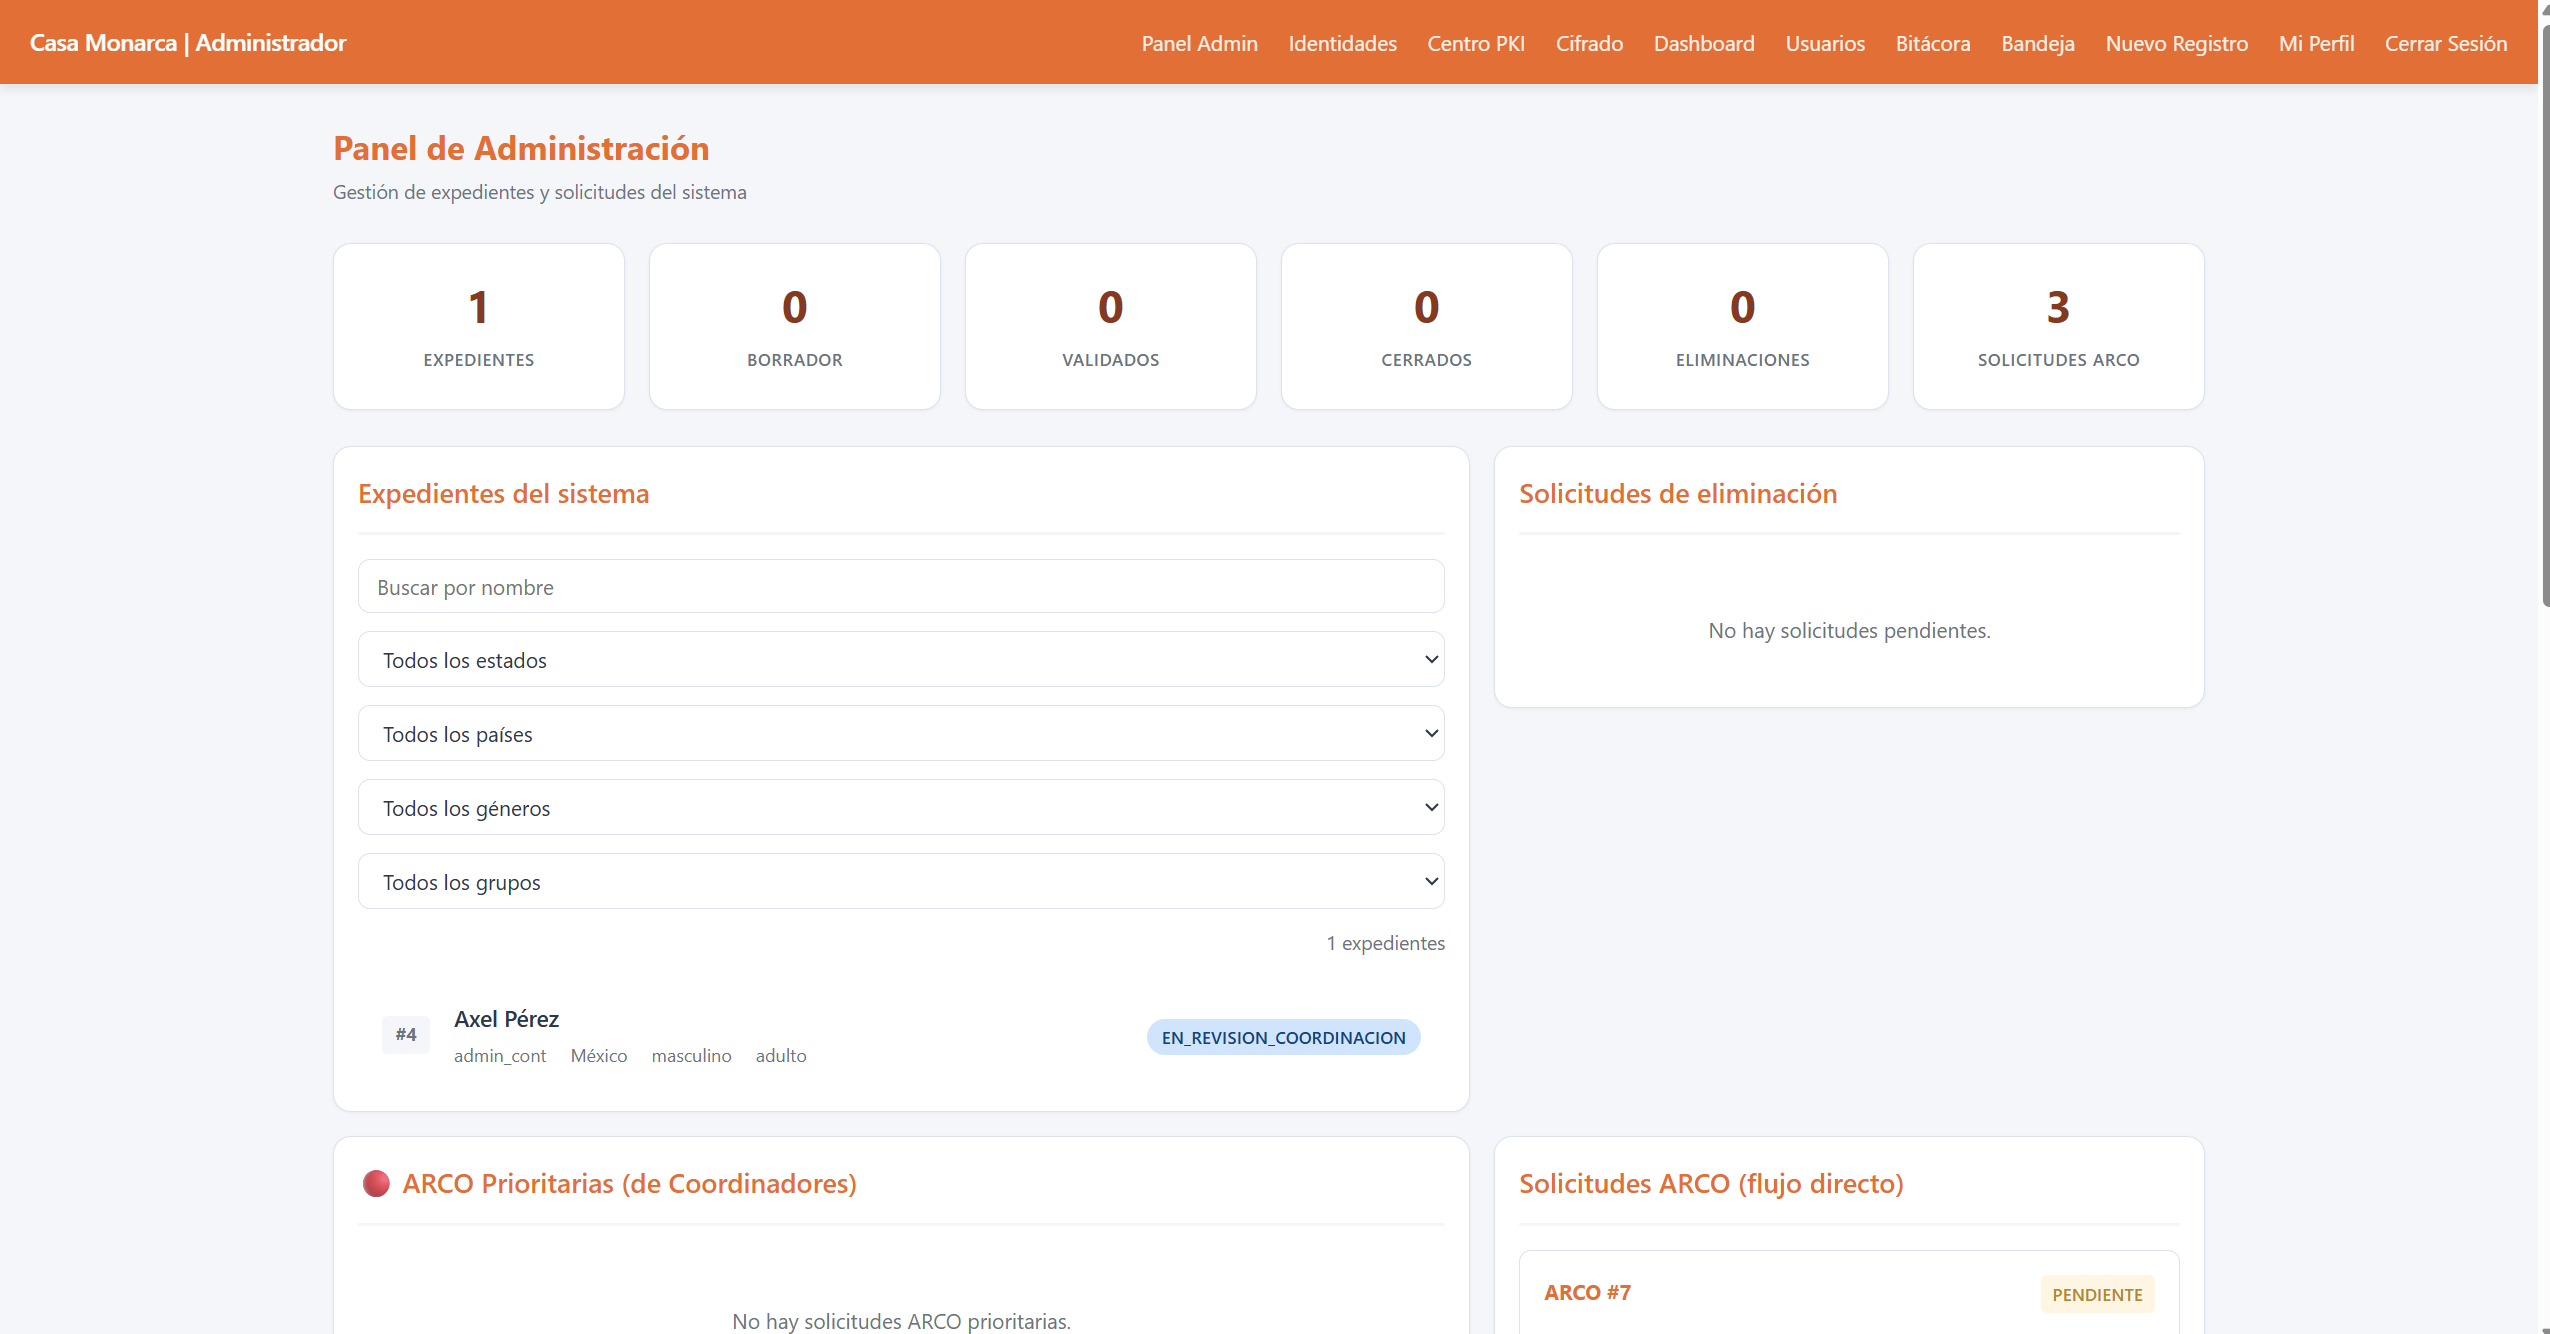
\includegraphics[width=0.8\textwidth]{Panel Admin.png}
  \end{minipage}
  \caption{Panel Admin}
  \label{fig:panel-admin}
\end{figure}

El \textbf{Panel de Administración} está reservado a los administradores y
concentra la gestión global de expedientes y solicitudes.

\subsection{Expedientes del sistema}

Muestra el listado completo de expedientes registrados, con su estado, para
que el administrador pueda supervisarlos.

\subsection{Solicitudes de eliminación}

Lista las solicitudes de eliminación generadas por otros usuarios. El
administrador puede aprobarlas o rechazarlas.

% ════════════════════════════════════════════════════════════════════
\section{Gestión de Usuarios}

La sección \textbf{Usuarios} (disponible para administradores) permite
administrar las cuentas de los colaboradores.

\subsection{Usuarios activos}

Muestra la lista de cuentas existentes con su rol y área. Junto a cada
usuario aparece el botón \textbf{Eliminar} para dar de baja la cuenta.

\begin{nota}[Verificación al eliminar]
La eliminación de un usuario requiere verificación confirmación, la identidad del admin queda guardada en la bitácora.
\end{nota}

\subsection{Crear nuevo usuario}

El formulario \textbf{Crear Nuevo Usuario} permite registrar una cuenta nueva
indicando usuario, contraseña, rol y área.

\begin{nota}[Verificación de identidad]
Al crear cuentas de Administrador o Coordinador, el sistema solicita una
\textbf{verificación de identidad con passkey} adicional antes de completar
el alta.
\end{nota}

\subsection{Eventos recientes y certificados}

La misma pantalla muestra los \textbf{eventos recientes} relacionados con
usuarios y un apartado de \textbf{certificados digitales}, donde es posible
\textbf{descargar} o \textbf{revocar} certificados asociados. Ambas
operaciones requieren verificación con passkey.

\begin{figure}[H]
  \centering
  \begin{minipage}{0.48\textwidth}
    \centering
    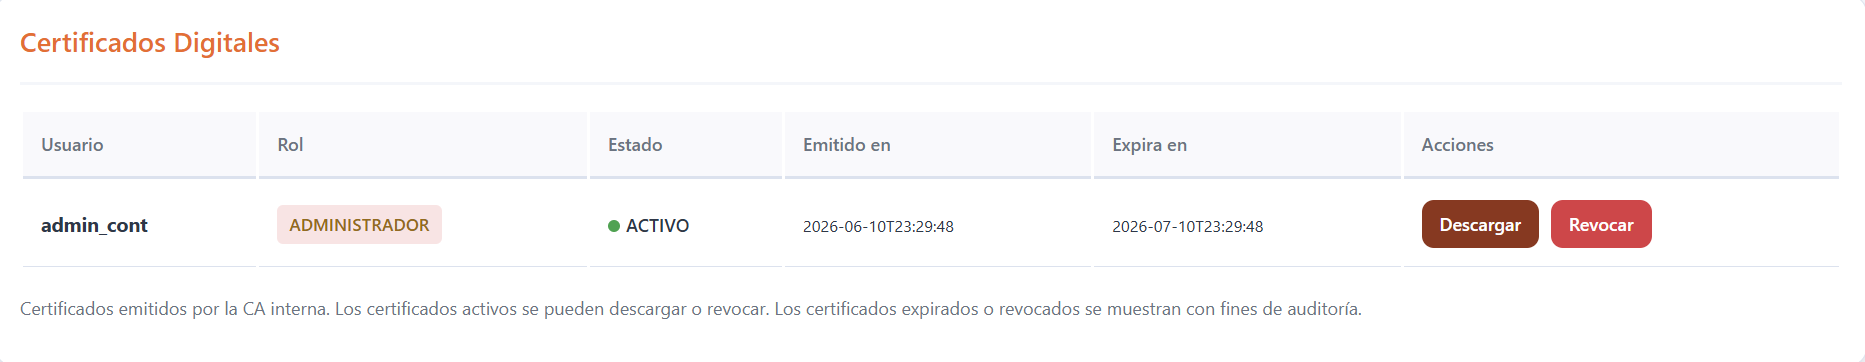
\includegraphics[width=0.8\textwidth]{Certificados Digitales.png}
  \end{minipage}
  \caption{Certificados Digitales}
  \label{fig:Certificados Digitales}
\end{figure}
\newpage
% ════════════════════════════════════════════════════════════════════
\section{Mi Perfil}

La pantalla \textbf{Mi Perfil} permite a cada usuario consultar y actualizar
su información, así como gestionar sus opciones de seguridad.

\begin{figure}[H]
  \centering
  \begin{minipage}{0.48\textwidth}
    \centering
    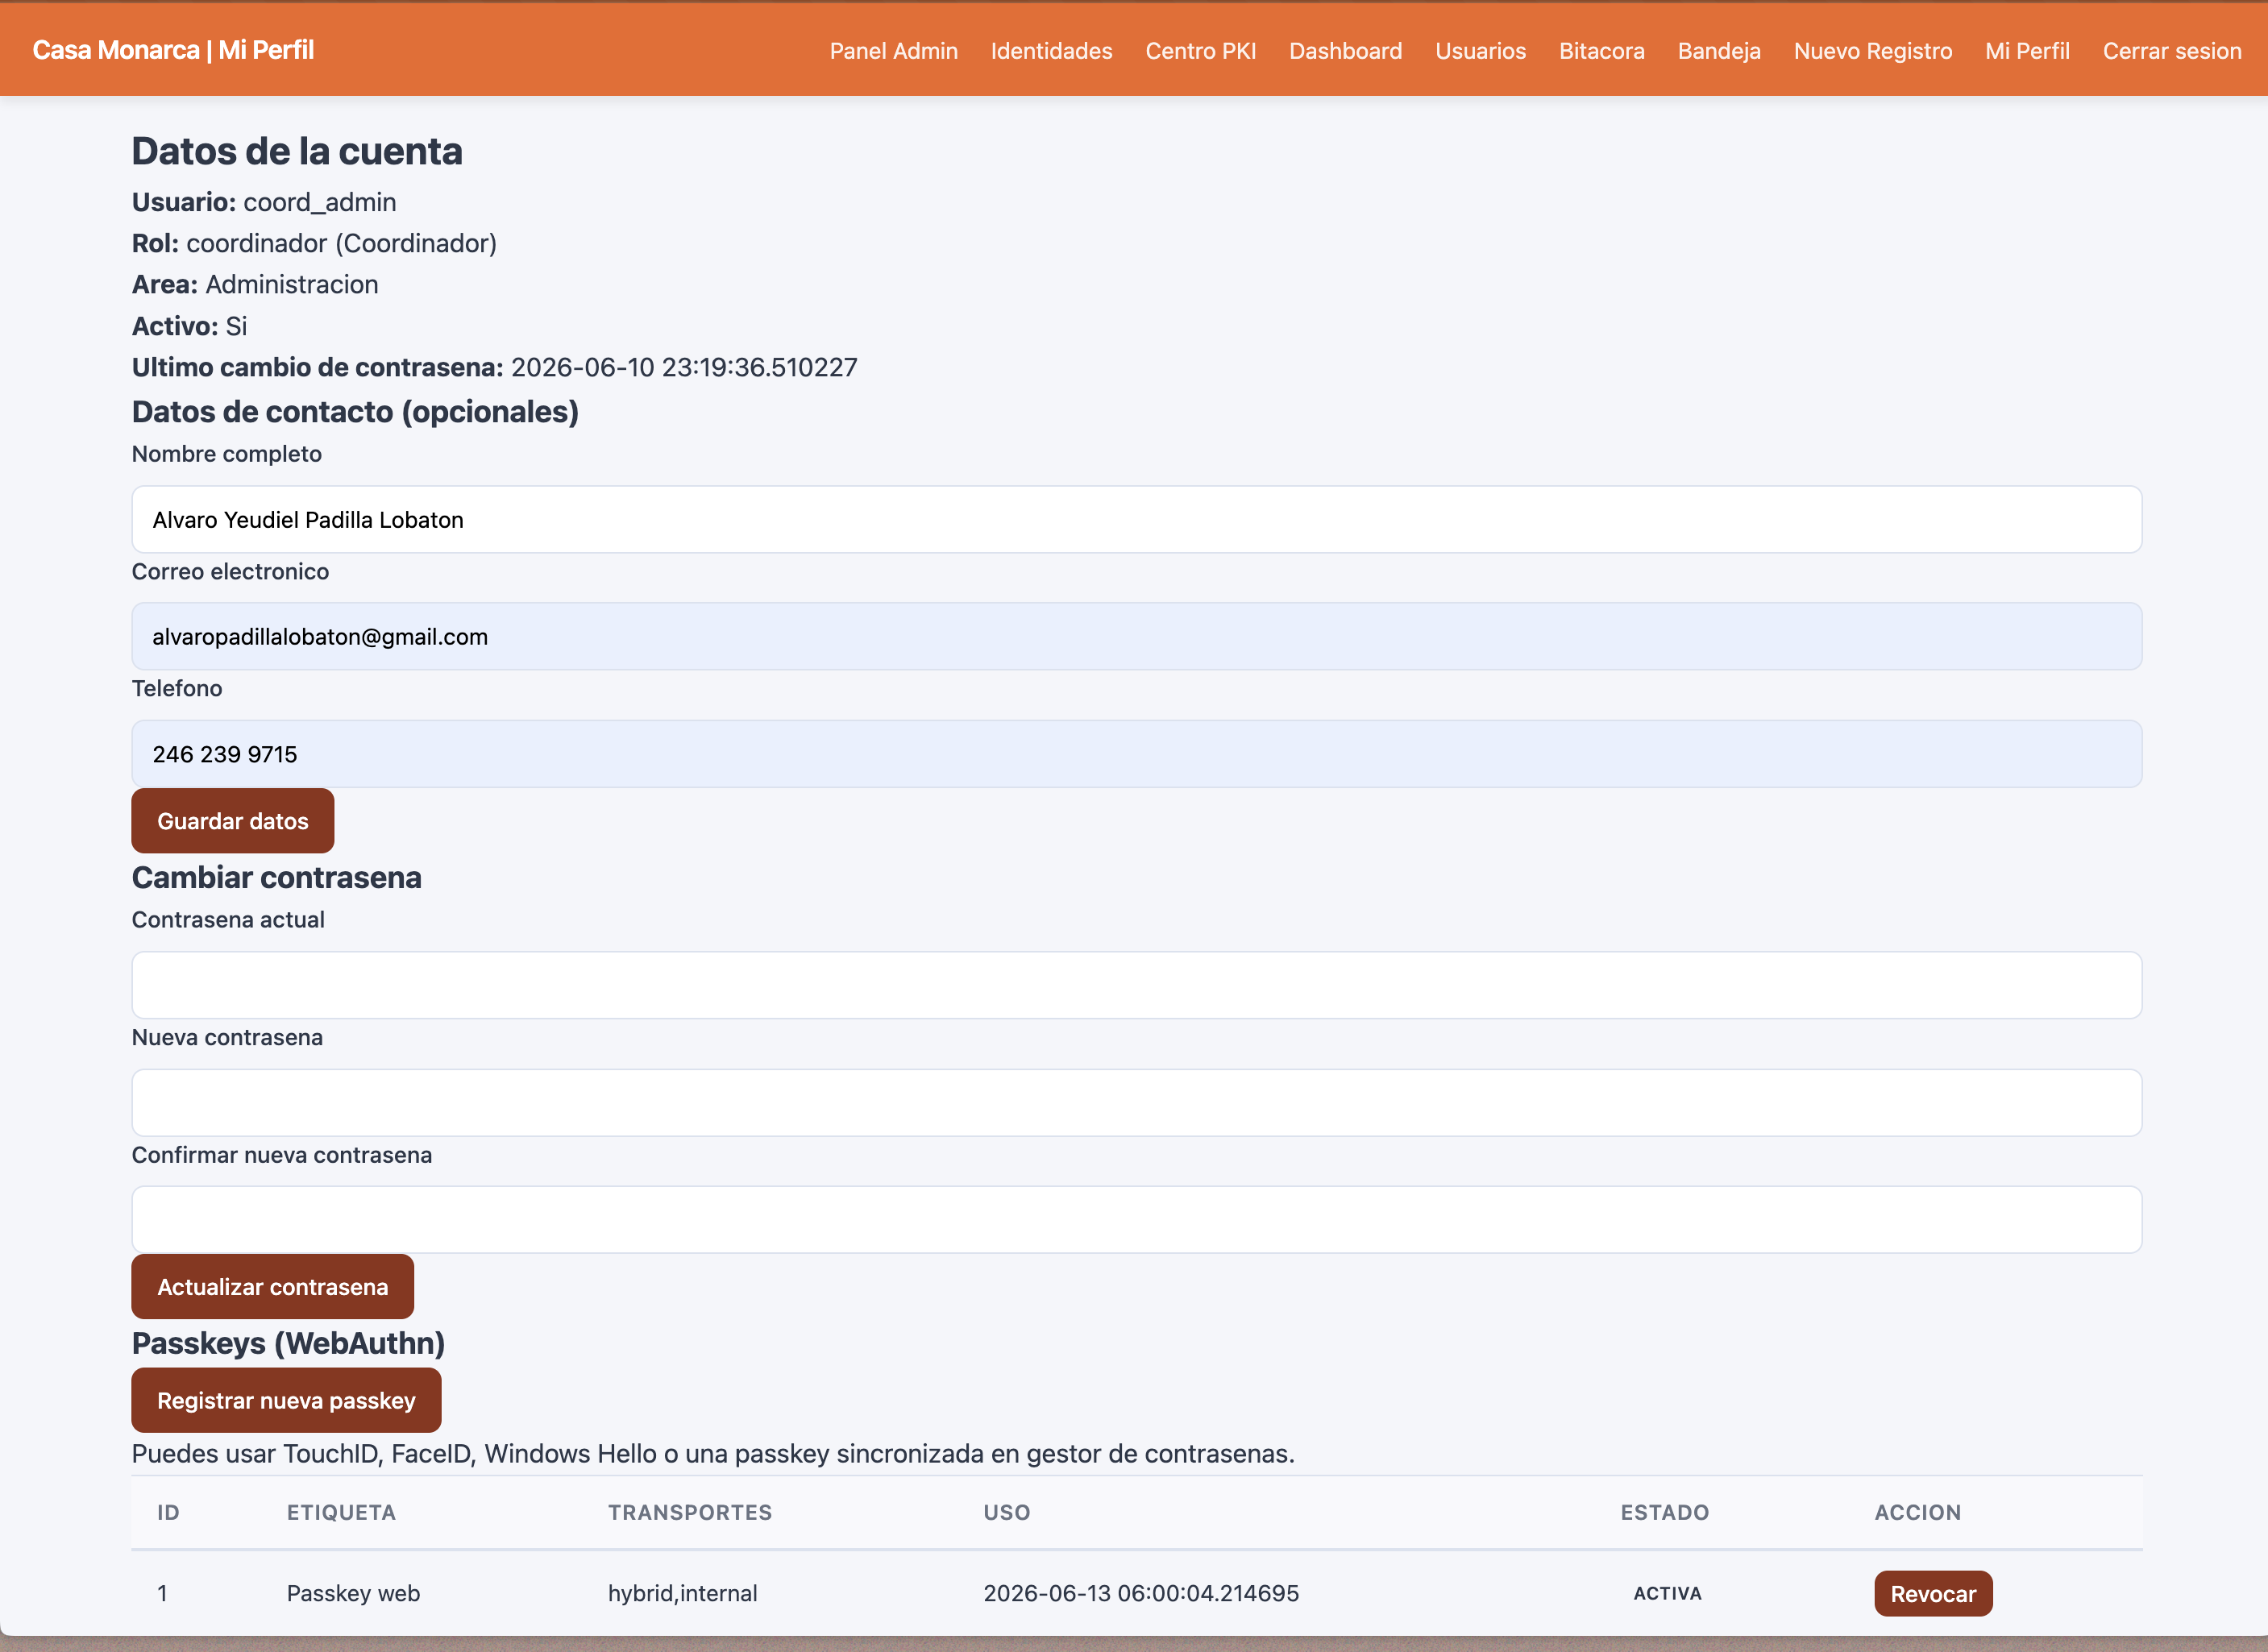
\includegraphics[width=0.8\textwidth]{Miperfil.png}
  \end{minipage}
  \caption{Visualización de Mi perfil}
  \label{fig:mi-perfil}
\end{figure}

\subsection{Datos de la cuenta}

Muestra la información básica de la cuenta (usuario, rol y área).

\subsection{Datos de contacto}

Permite registrar datos opcionales como nombre completo, correo electrónico y
teléfono. Presione \textbf{Guardar datos} para conservar los cambios.

\subsection{Cambiar contraseña}

Desde este apartado el usuario puede actualizar su contraseña en cualquier
momento, escribiendo la nueva clave y confirmándola con \textbf{Actualizar
contraseña}.

\subsection{Passkeys (WebAuthn)}

Permite administrar las llaves de acceso del usuario:

\begin{itemize}[leftmargin=2em]
  \item \textbf{Registrar nueva passkey:} vincula un nuevo método de acceso
    (huella, rostro o PIN del dispositivo).
  \item \textbf{Revocar:} desactiva una passkey existente.
\end{itemize}

\begin{figure}[H]
  \centering
  \begin{minipage}{0.48\textwidth}
    \centering
    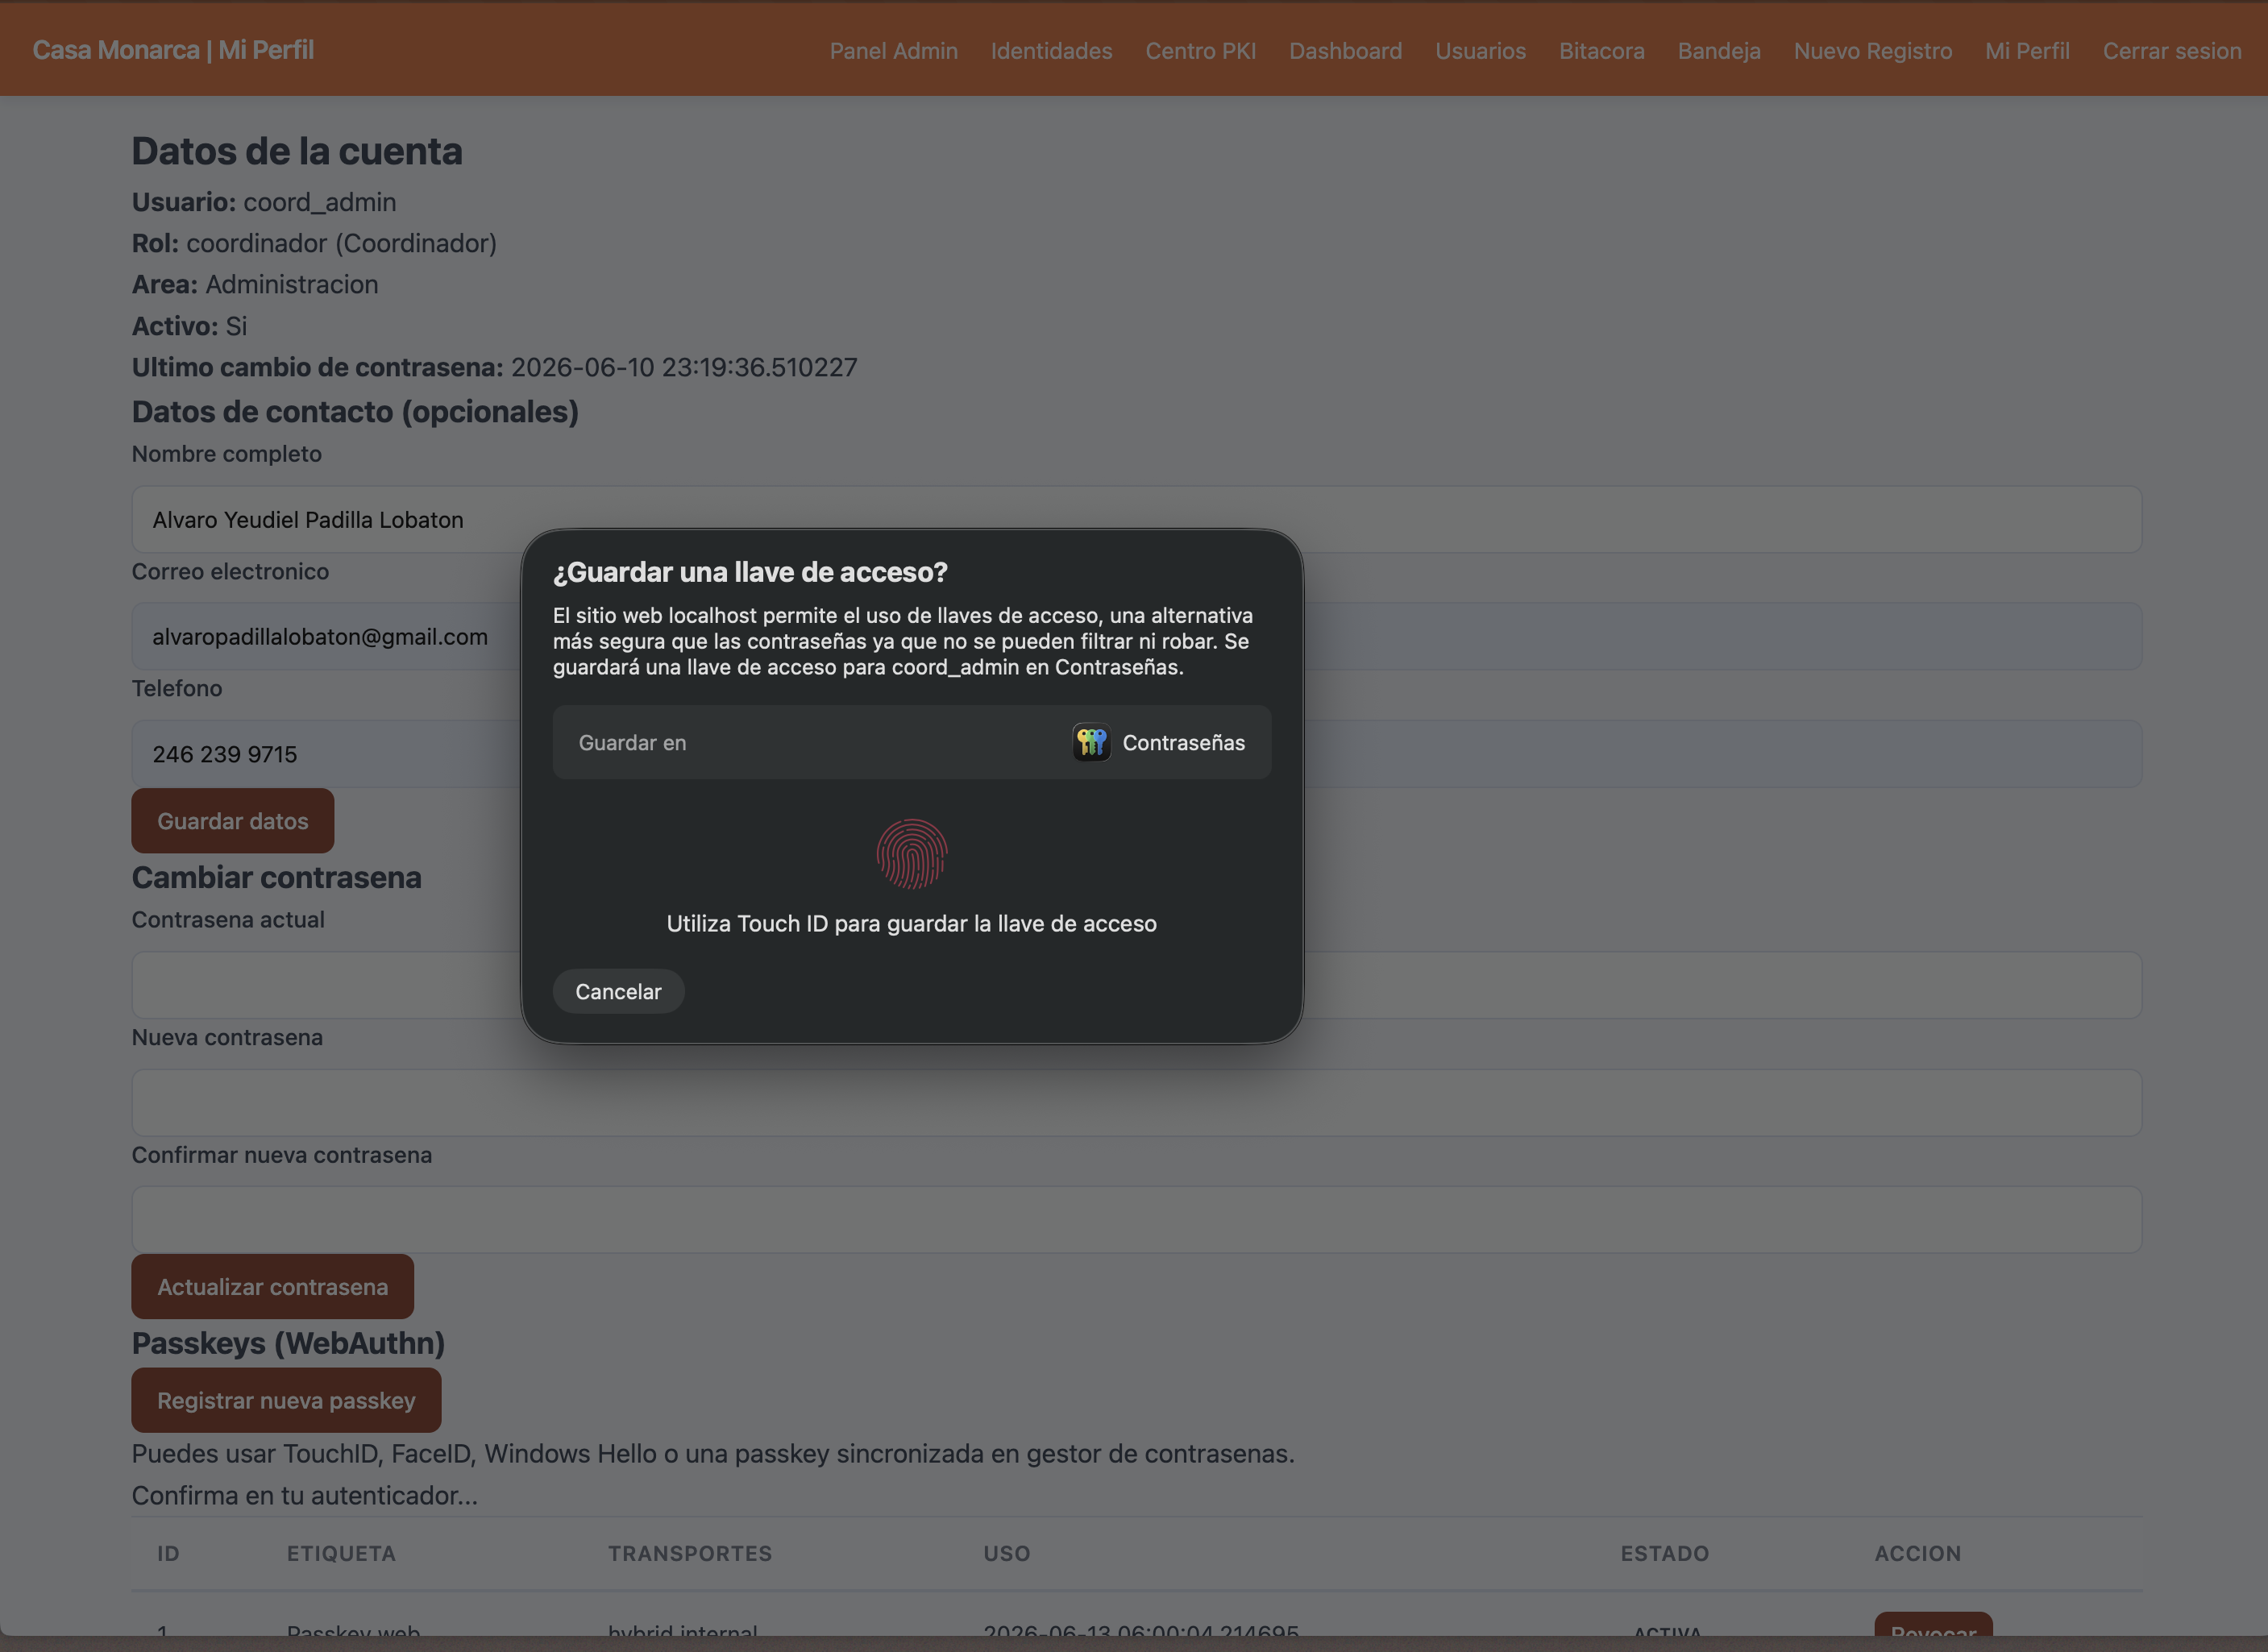
\includegraphics[width=0.8\textwidth]{RegistroNueva.png}
  \end{minipage}
  \caption{Registrar Nueva Passkey}
  \label{fig:registro-passkey}
\end{figure}

% ════════════════════════════════════════════════════════════════════
\section{Bitácora de Eventos}

La \textbf{Bitácora} registra todas las acciones relevantes realizadas en el
sistema: inicios de sesión, creación y movimiento de expedientes, cambios de
configuración y acciones de seguridad.

\begin{figure}[H]
  \centering
  \begin{minipage}{0.48\textwidth}
    \centering
    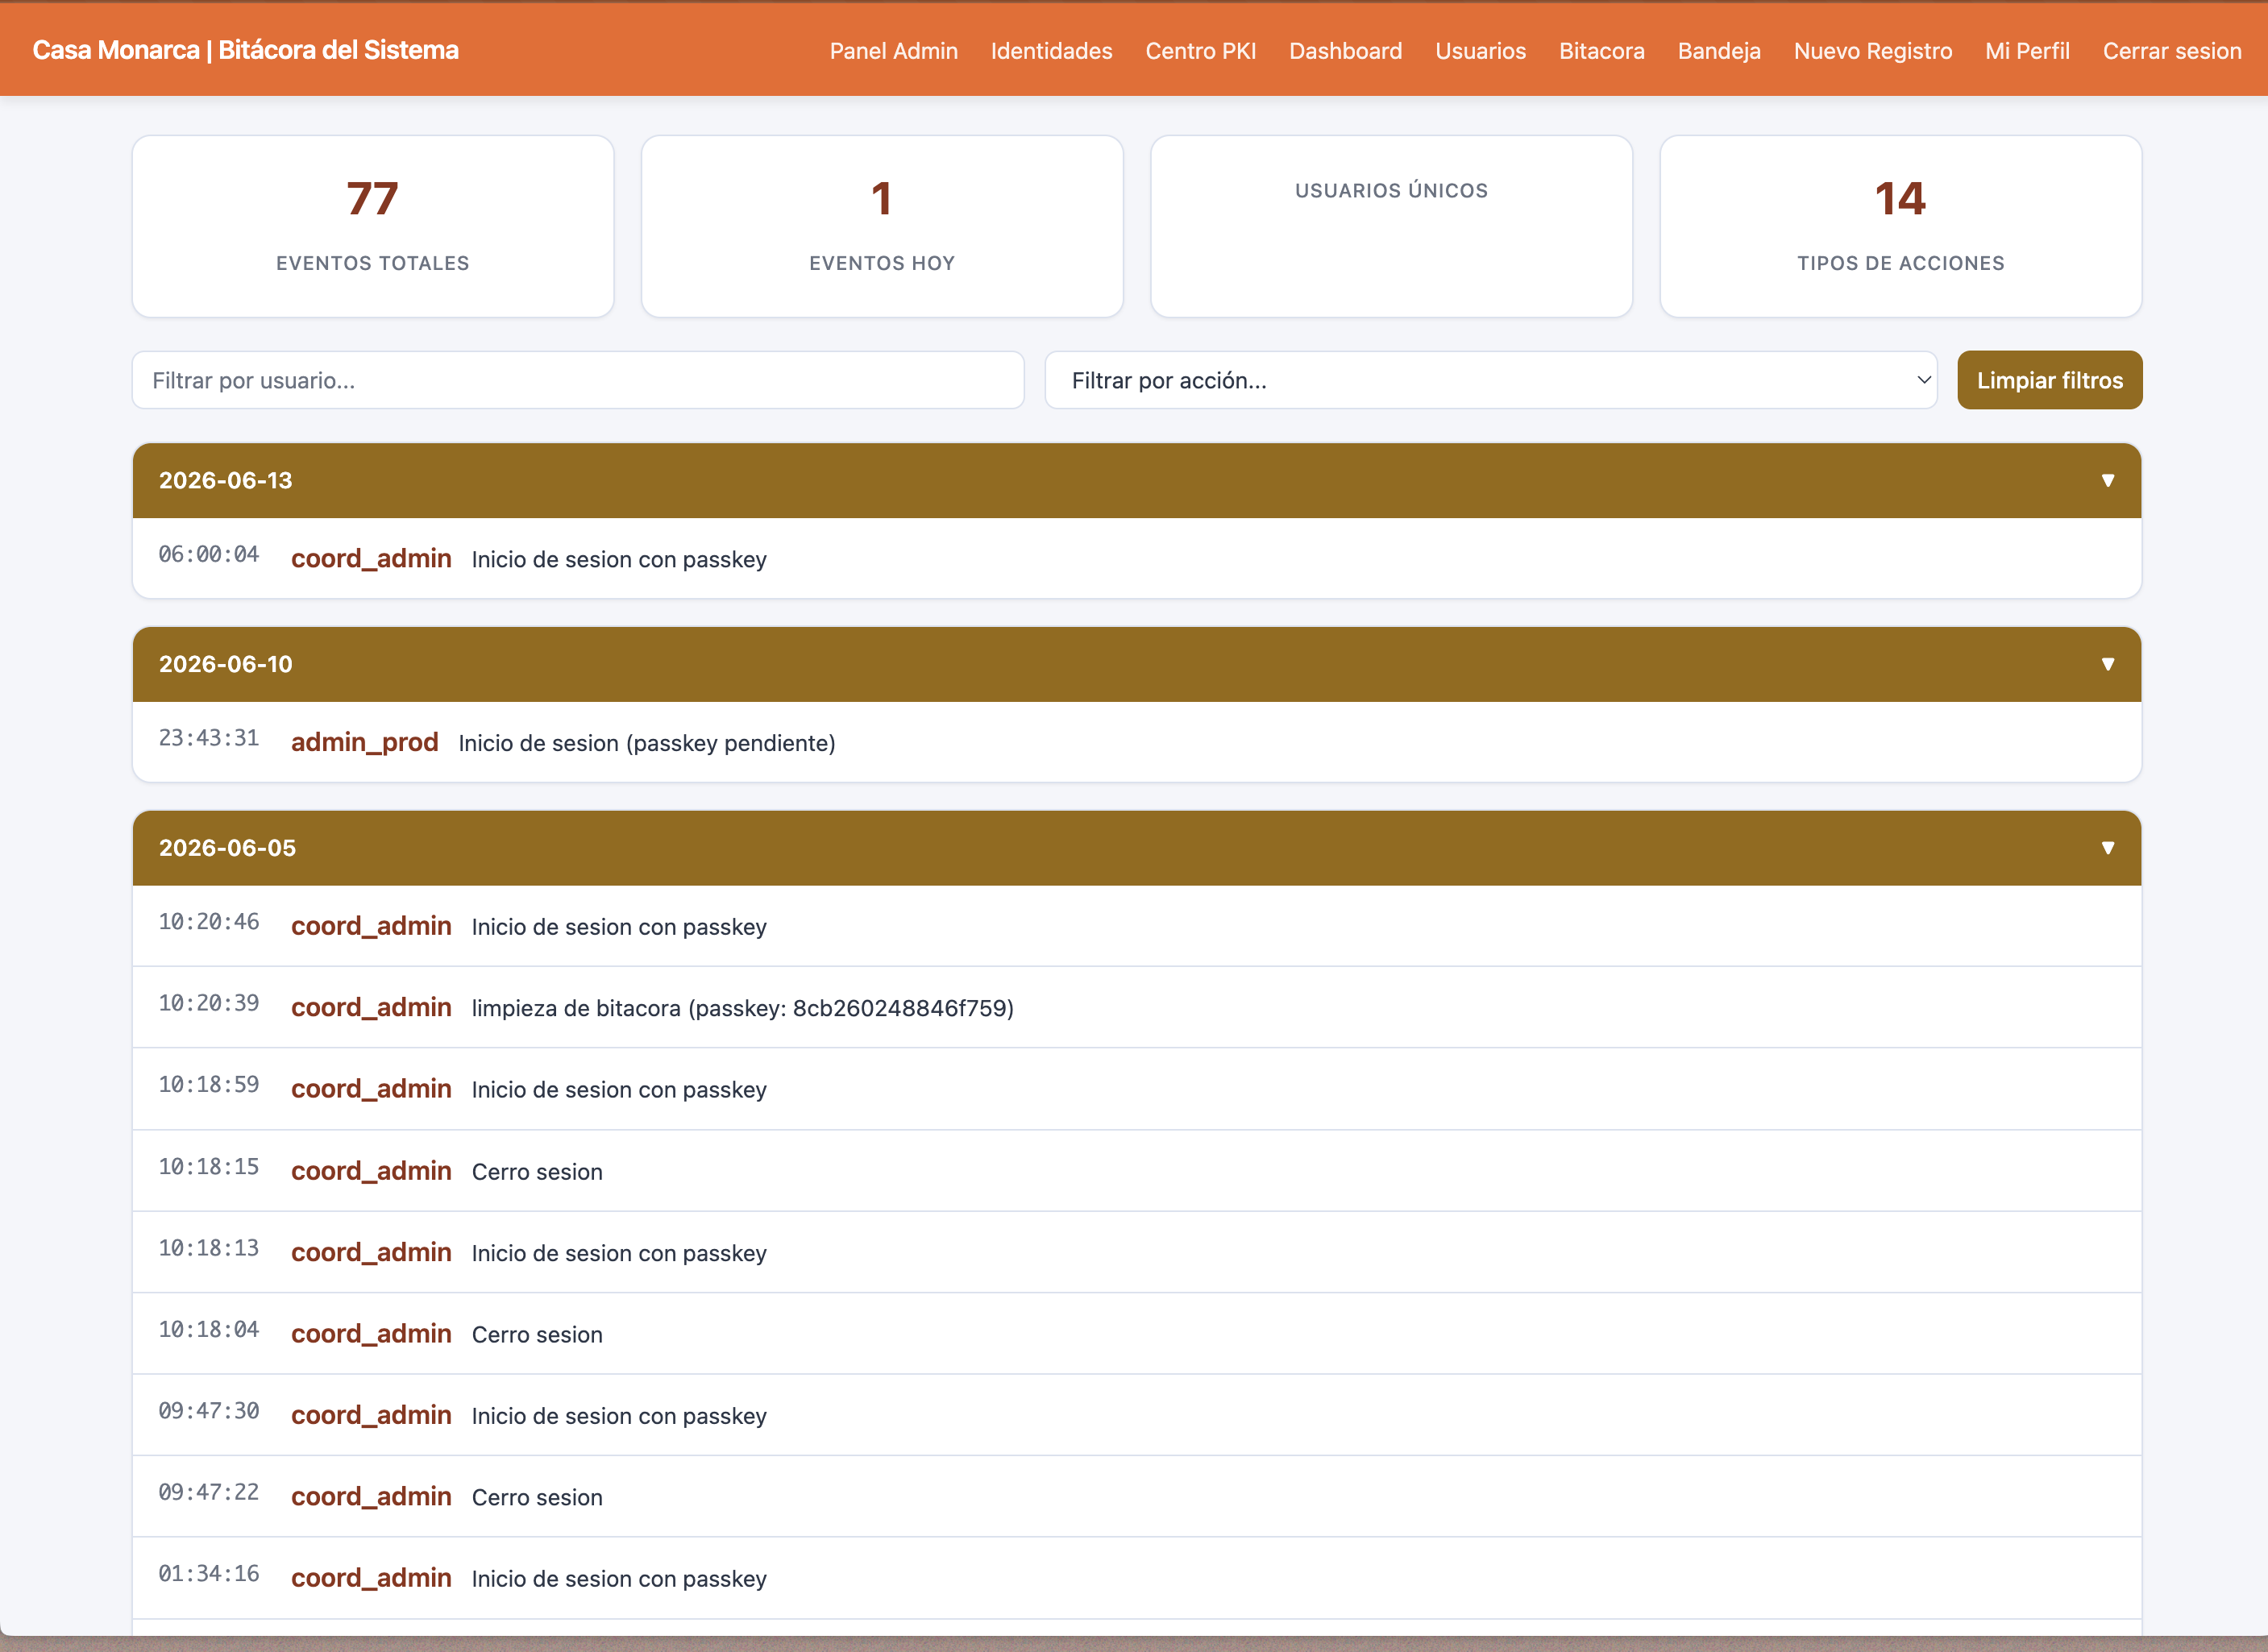
\includegraphics[width=0.8\textwidth]{Bitacora.png}
  \end{minipage}
  \caption{Visualización de la Bitácora}
  \label{fig:bitacora}
\end{figure}

\subsection{Consulta y filtros}

La bitácora permite filtrar los eventos (por ejemplo, por usuario, categoría
o fecha) para localizar información específica. El botón \textbf{Limpiar
filtros} restablece la vista completa.

\subsection{Mantenimiento}

Los administradores pueden depurar la bitácora cuando sea necesario mediante
la opción de limpieza disponible en la pantalla.

% ════════════════════════════════════════════════════════════════════
\section{Centro de Control PKI}

El \textbf{Centro de Control PKI} (administradores) gestiona los certificados
digitales que respaldan la identidad de los usuarios críticos.

\begin{figure}[H]
  \centering
  \begin{minipage}{0.48\textwidth}
    \centering
    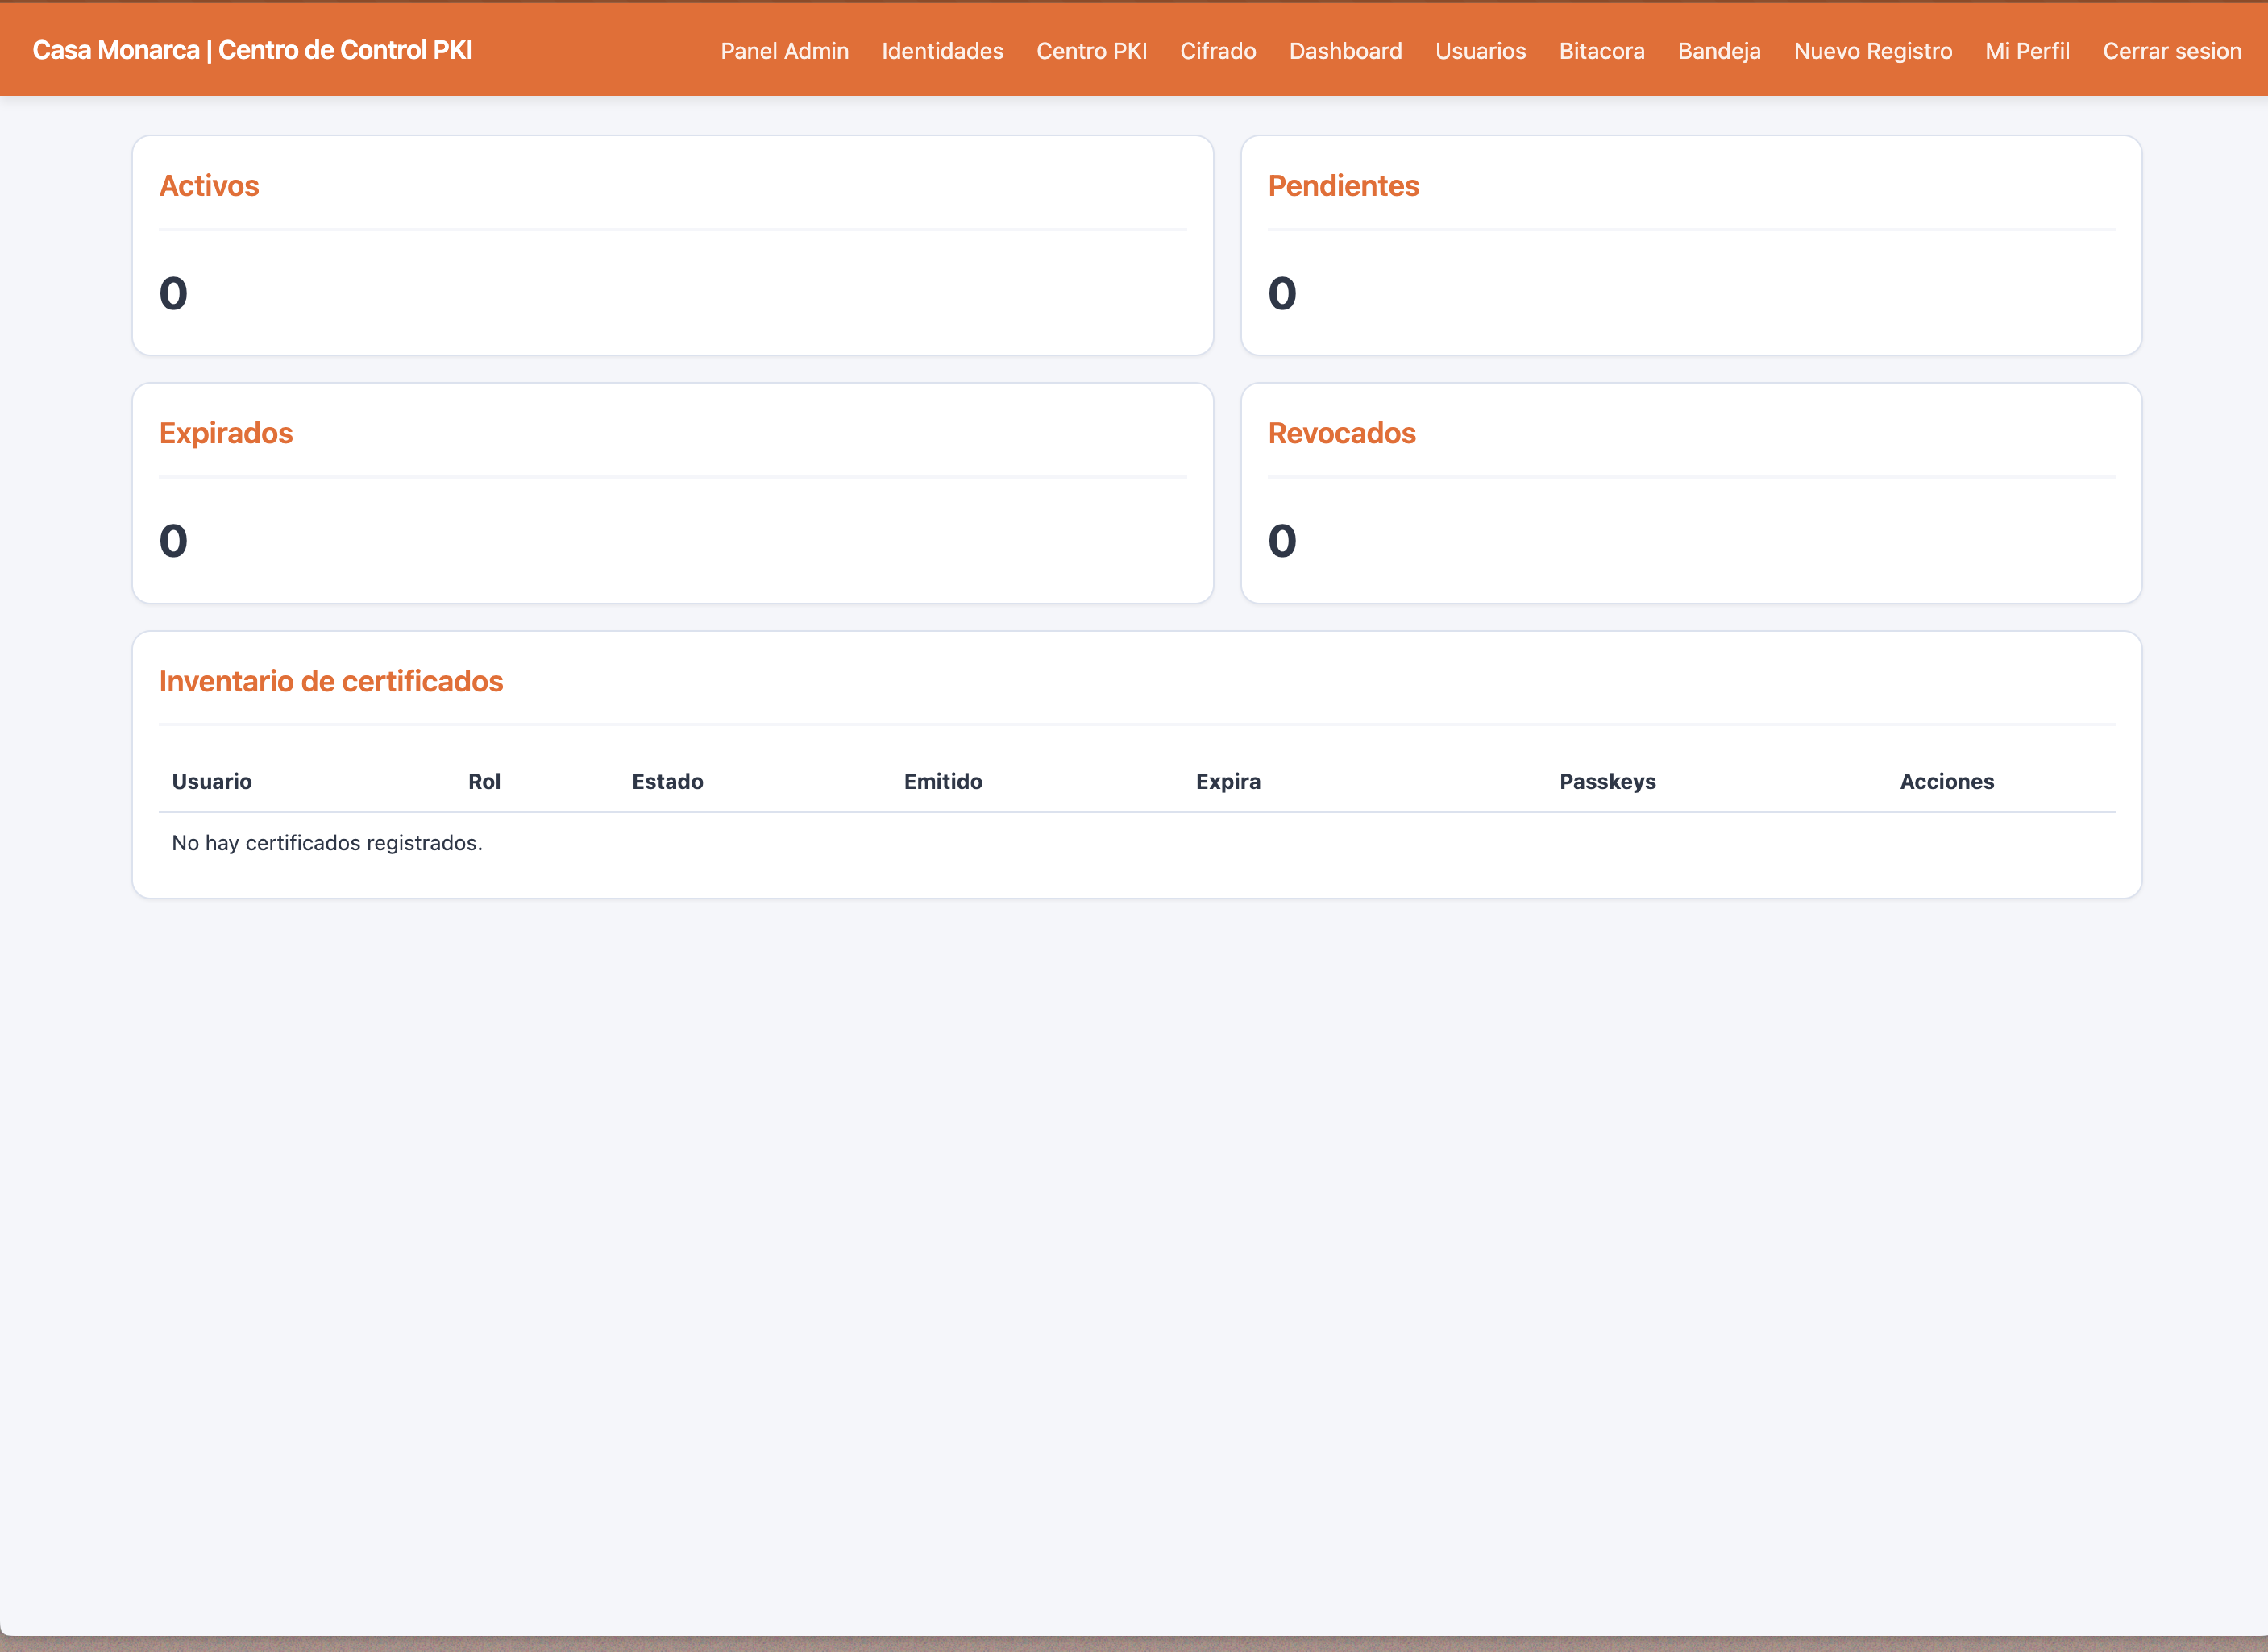
\includegraphics[width=0.8\textwidth]{CentroPKI.png}
  \end{minipage}
  \caption{Visualización del Centro PKI}
  \label{fig:centro-pki}
\end{figure}

\subsection{Resumen de certificados}

En la parte superior se muestran contadores con el estado de los
certificados: \textbf{Activos}, \textbf{Pendientes}, \textbf{Expirados} y
\textbf{Revocados}.

\subsection{Inventario de certificados}

Lista todos los certificados emitidos. Para cada uno se puede:

\begin{itemize}[leftmargin=2em]
  \item Ver los \textbf{Detalles} del certificado (vigencia, huella, passkeys
    vinculadas).
  \item \textbf{Descargar} el certificado en formato PEM
    (requiere verificación con passkey).
  \item \textbf{Revocar} el certificado cuando ya no deba ser válido
    (requiere verificación con passkey).
\end{itemize}

% ════════════════════════════════════════════════════════════════════
\section{Panel de Cifrado}
\label{sec:cifrado}

El Panel de Cifrado está disponible para Administradores y Coordinadores. Permite gestionar las llaves de cifrado AES-256 con las que se protegen todos los expedientes almacenados en el sistema.

\subsection{Inventario de cifrado}

Al ingresar, la pantalla muestra el inventario actual de cifrado:
el número de registros cifrados, la llave activa y su huella digital
(\textit{fingerprint}).

\begin{figure}[H]
  \centering
  \begin{minipage}{0.48\textwidth}
    \centering
    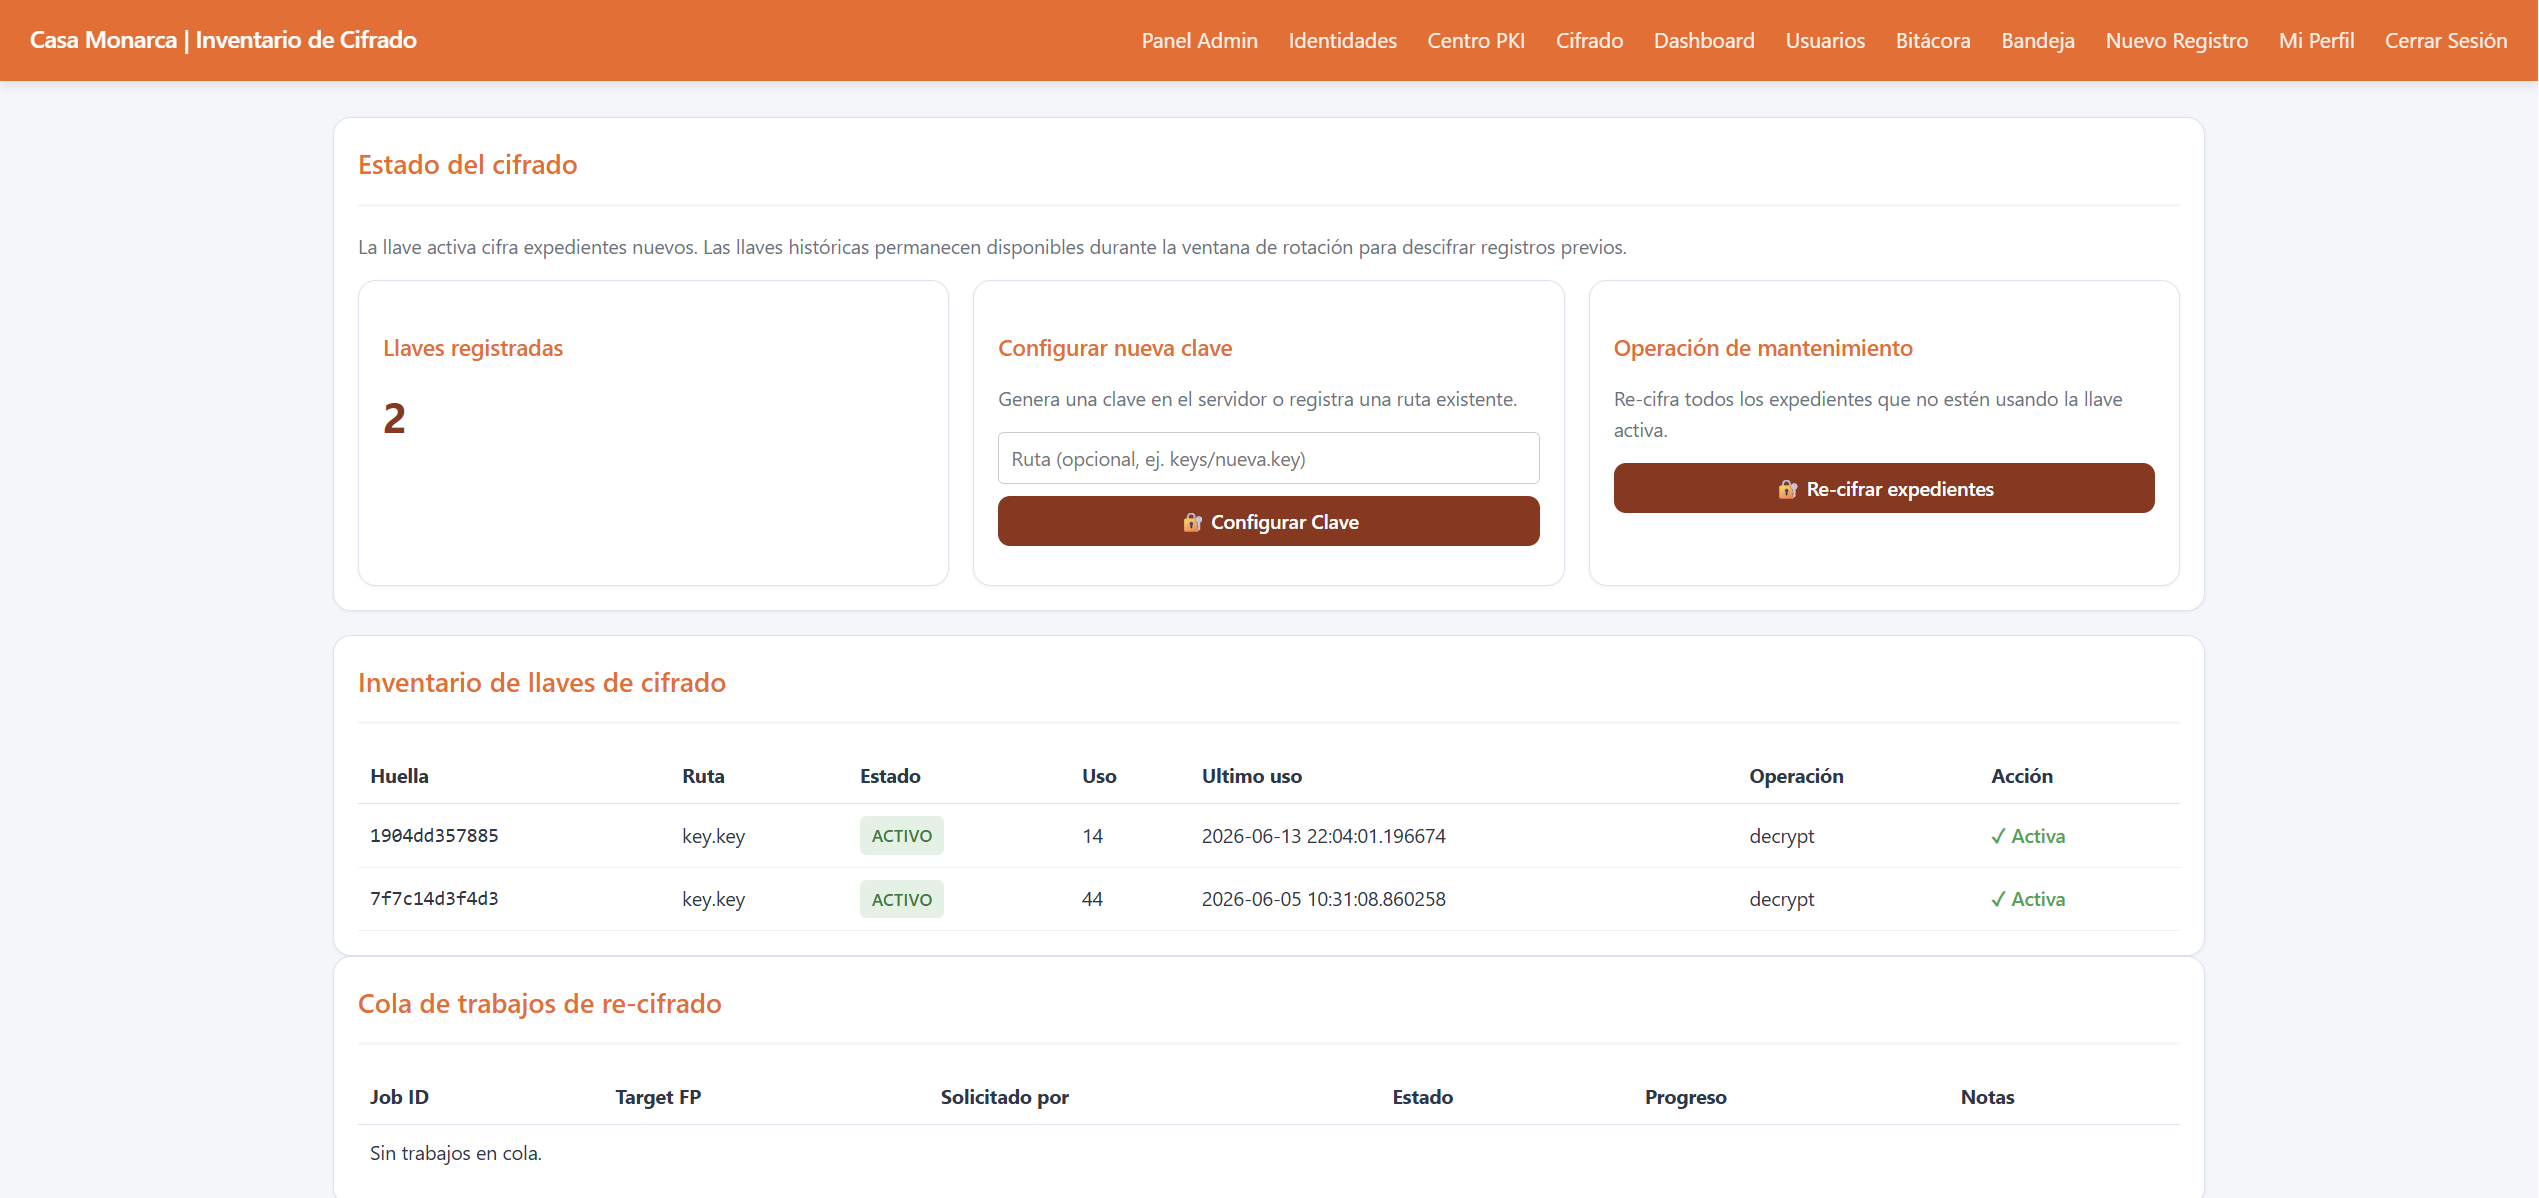
\includegraphics[width=0.8\textwidth]{Inventario de Cifrado.png}
  \end{minipage}
  \caption{Inventario de Cifrado}
  \label{fig:centro-pki}
\end{figure}

\subsection{Configurar una nueva llave}

Para registrar una nueva llave de cifrado:

\begin{enumerate}[leftmargin=2em]
  \item Ingrese o pegue la llave Fernet en el campo correspondiente, o
    utilice la opción de generación automática.
  \item Presione \textbf{Guardar llave}.
  \item La llave quedará registrada pero \textit{inactiva} hasta que se
    active explícitamente.
\end{enumerate}

\subsection{Activar una llave}

Para que una llave proteja los nuevos registros:

\begin{enumerate}[leftmargin=2em]
  \item Localice la llave deseada en el listado.
  \item Presione \textbf{Activar}.
  \item Complete la \textbf{verificación con passkey}
    (véase sección~\ref{sec:passkey-action}).
\end{enumerate}

\begin{nota}[Re-cifrado automático]
Al activar una nueva llave, el sistema inicia automáticamente un trabajo de
re-cifrado que convierte todos los expedientes existentes a la nueva llave.
Este proceso puede tardar varios minutos dependiendo del volumen de datos.
\end{nota}

\subsection{Re-cifrado masivo}

Si necesita forzar el re-cifrado de todos los expedientes con la llave
activa actual:

\begin{enumerate}[leftmargin=2em]
  \item Presione \textbf{Re-cifrar todos los expedientes}.
  \item Complete la verificación con passkey.
  \item El sistema mostrará cuántos registros fueron actualizados y cuántos
    fueron omitidos (ya estaban cifrados con la llave activa).
\end{enumerate}

\subsection{Monitoreo de trabajos de re-cifrado}

La pantalla muestra en tiempo real el estado de los trabajos de re-cifrado
en progreso, incluyendo cuántos registros han sido procesados del total.
También se pueden consultar las métricas de rendimiento de operaciones de
cifrado (tiempo promedio, llaves utilizadas, historial de operaciones).

\begin{figure}[H]
  \centering
  \begin{minipage}{0.48\textwidth}
    \centering
    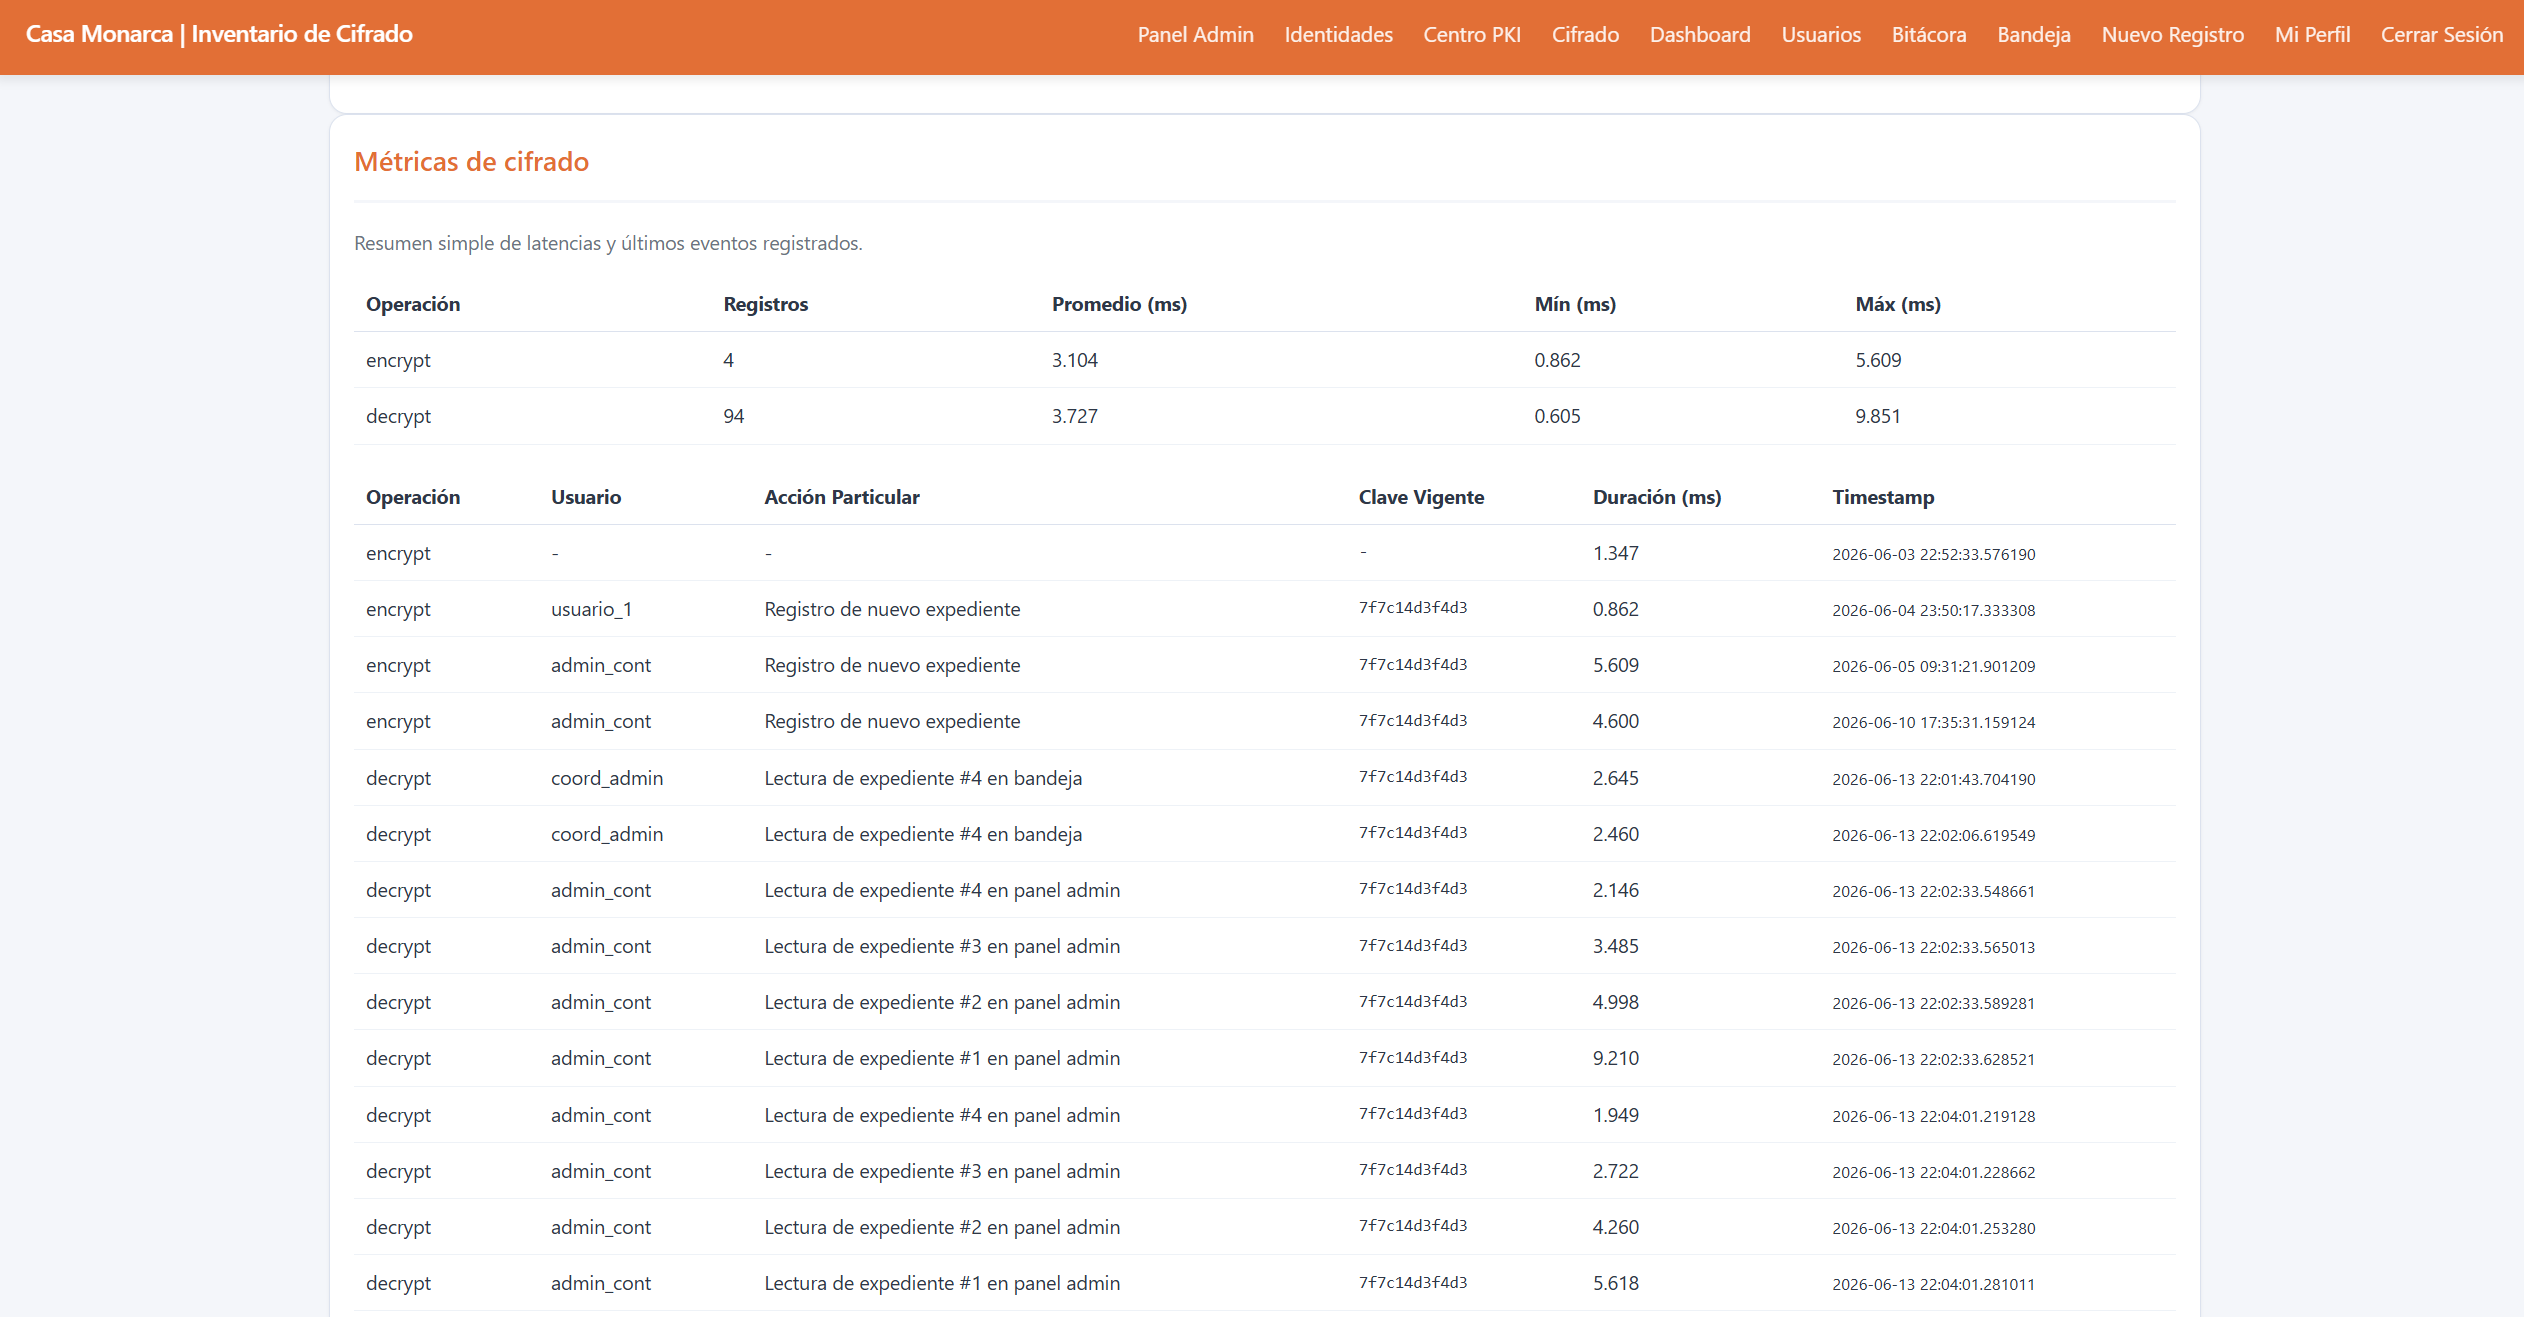
\includegraphics[width=0.8\textwidth]{Inventario de Cifrados.png}
  \end{minipage}
  \caption{Bitacora de Cifrado}
  \label{fig:centro-pki}
\end{figure}

\begin{nota}[Acceso de coordinadores]
Los coordinadores pueden consultar el inventario de cifrado y las métricas,
pero las operaciones de activación y re-cifrado requieren adicionalmente la
verificación con passkey.
\end{nota}

% ════════════════════════════════════════════════════════════════════
\section{Gestión de Identidades}

La pantalla \textbf{Identidades} ofrece a los administradores una vista consolidada de las identidades digitales de los usuarios del sistema. Muestra, para cada cuenta, su rol, área, estado del certificado asociado y las passkeys registradas, permitiendo detectar rápidamente cuentas sin certificado activo o con passkeys sin vincular.

\begin{figure}[H]
  \centering
  \begin{minipage}{0.48\textwidth}
    \centering
    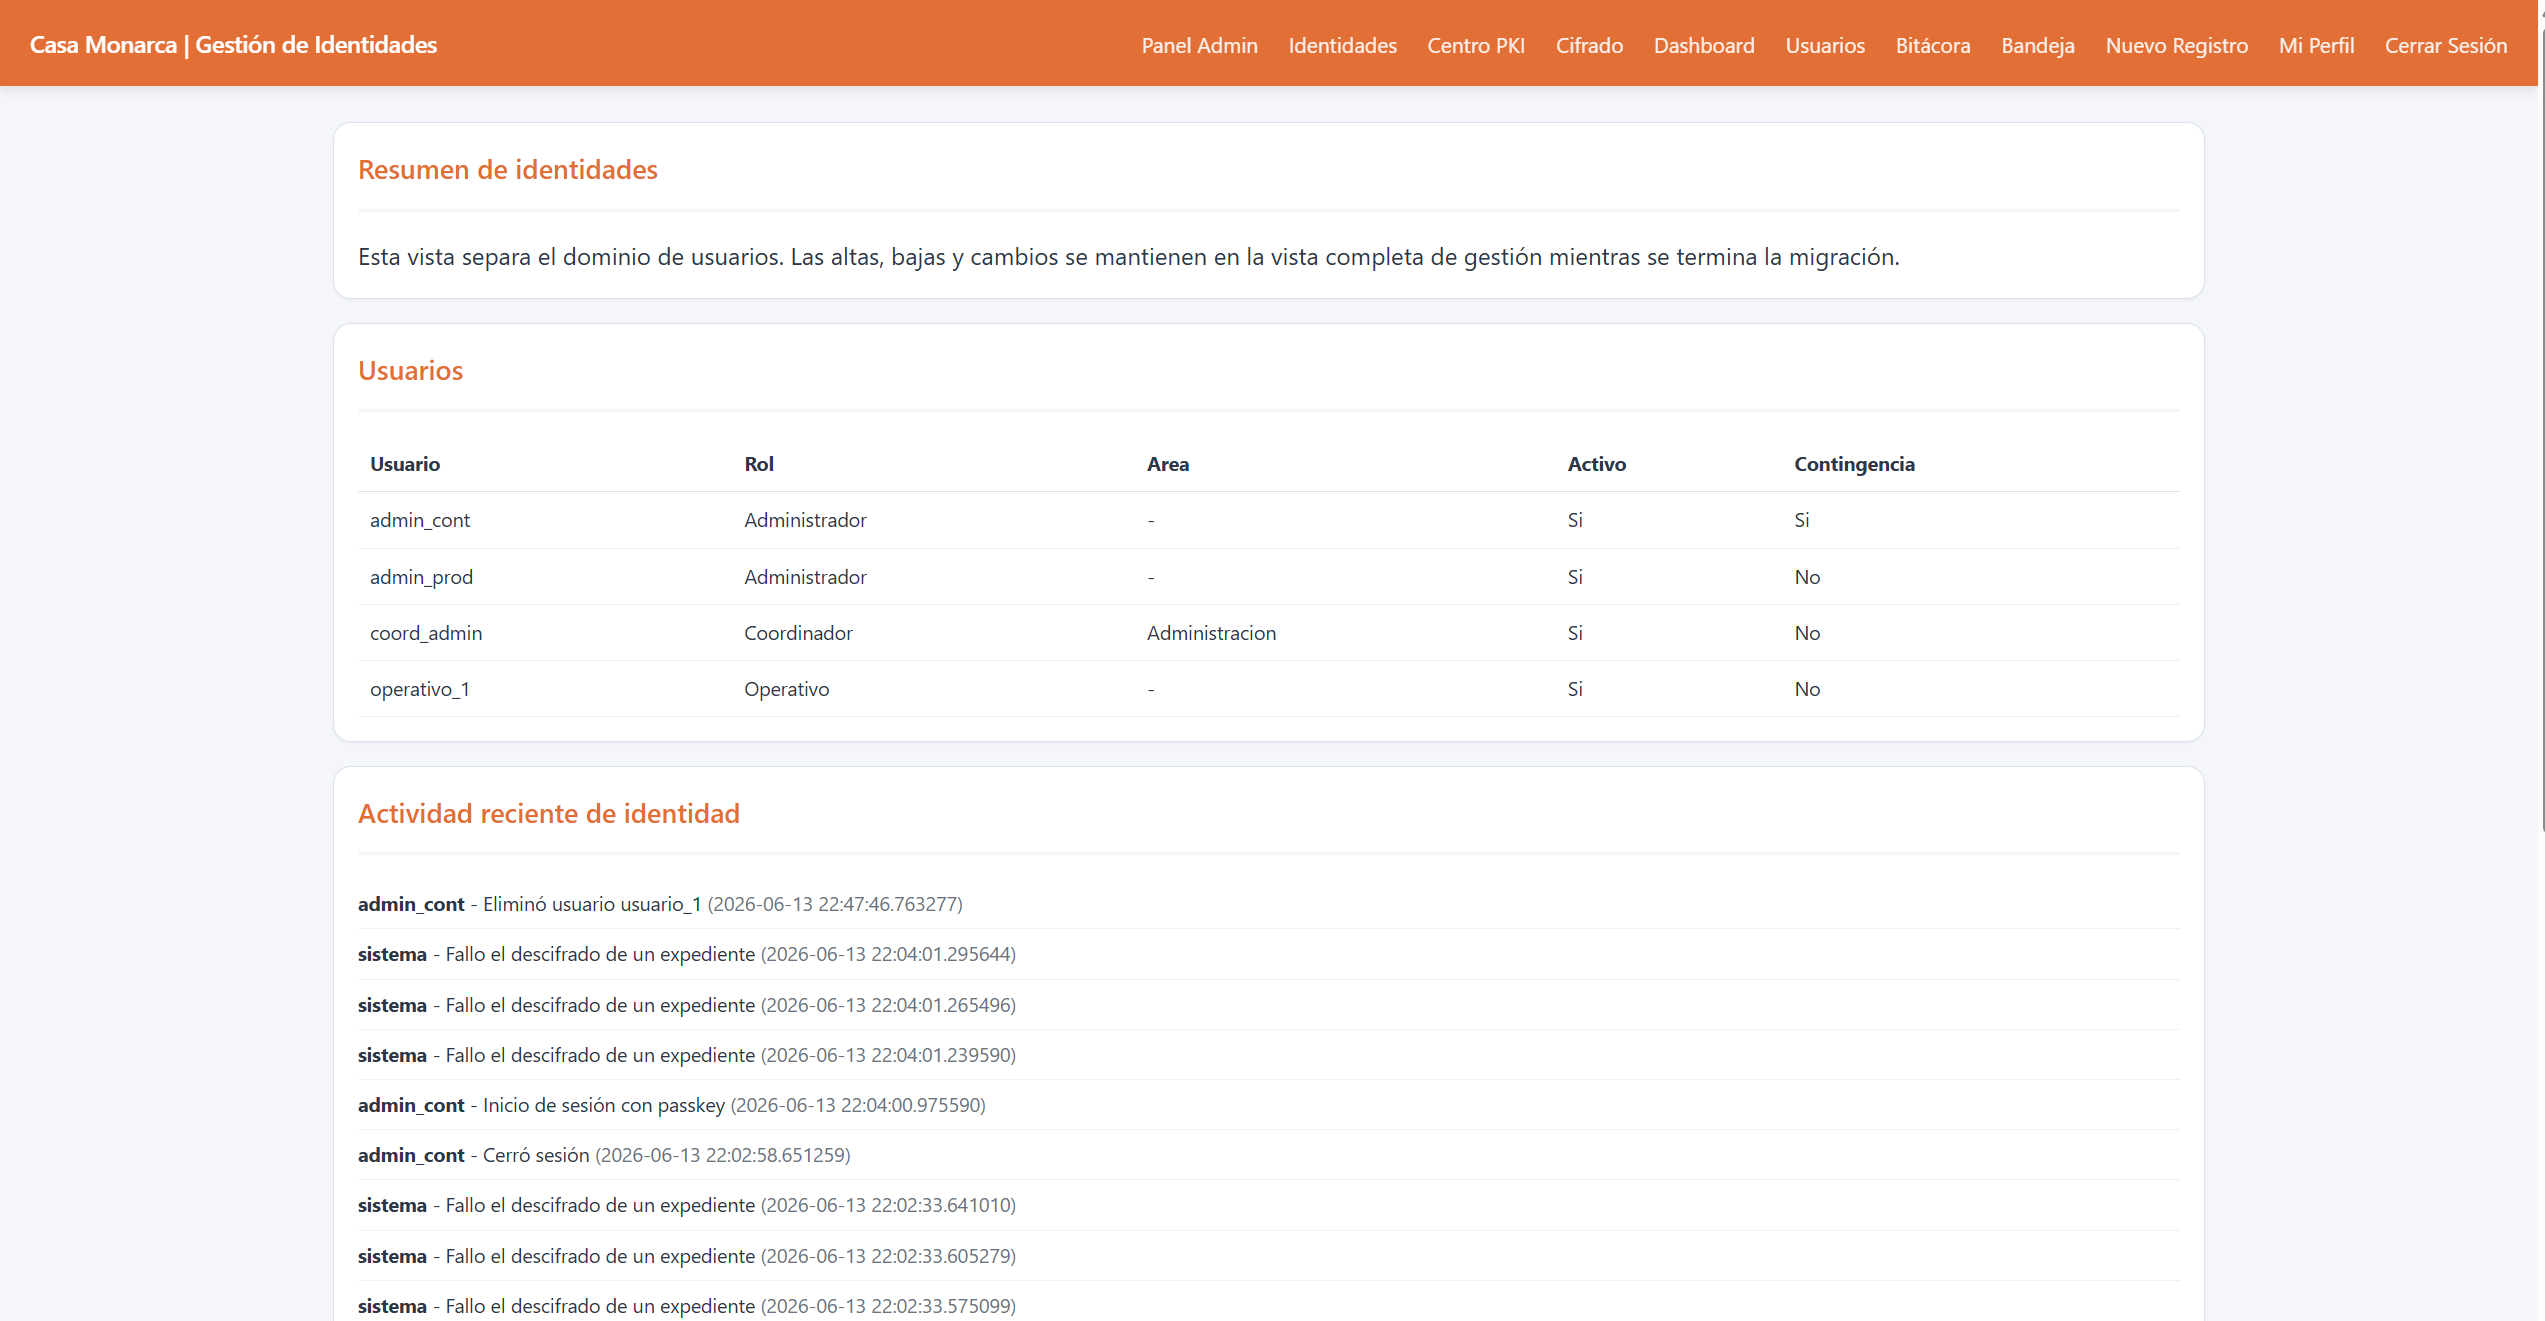
\includegraphics[width=0.8\textwidth]{Gestion de Identidades.png}
  \end{minipage}
  \caption{Bitacora de Cifrado}
  \label{fig:centro-pki}
\end{figure}

\section{Preguntas Frecuentes}

\subsubsection*{¿Qué hago si olvidé mi contraseña?}
Contacte al administrador del sistema para que restablezca su contraseña. No existe
recuperación automática por correo electrónico.

\subsubsection*{¿Por qué no puedo ver los datos de un expediente?}
Es posible que los datos estén cifrados con una llave diferente a la activa, o que su rol no tenga permisos para acceder a ese expediente. Contacte al administrador.

\subsubsection*{¿Qué pasa si se bloquea mi cuenta?}
Después de 5 intentos fallidos, la cuenta se bloquea 15 minutos. Espere y vuelva a
intentarlo, o contacte al administrador para desbloqueo manual.

\subsubsection*{¿Puedo usar el sistema desde mi teléfono?}
Sí, el sistema es compatible con navegadores móviles. Las passkeys también funcionan
en dispositivos Android e iOS modernos con autenticación biométrica.

\subsubsection*{¿Por qué se me pide mi passkey para ciertas acciones?}
Algunas acciones críticas (como activar una llave de cifrado, revocar certificados o
resolver solicitudes ARCO como coordinador) requieren una firma digital con passkey
para garantizar que fue usted quien autorizó la acción. Esta verificación tiene
validez de 5 minutos.

\end{document}